\documentclass{report}

\usepackage[english%,greek
]{babel}
\usepackage[T1]{fontenc}
\usepackage{notomath}
\usepackage{float}
\usepackage{color, colortbl}
\usepackage{placeins}
\usepackage{caption}
\usepackage{subcaption}
\usepackage{biblatex}
\addbibresource{references.bib}
\definecolor{gray}{gray}{0.9}
\definecolor{blue}{RGB}{82, 138, 174}
\usepackage[a4paper,top=2cm,bottom=2cm,left=3cm,right=3cm,marginparwidth=1.75cm]{geometry}
\usepackage{amsmath}
\usepackage{graphicx}
\usepackage[colorlinks=true, allcolors=blue]{hyperref}
\usepackage[export]{adjustbox}
\usepackage[none]{hyphenat}


\title{%Ενεργειακός Ισολογισμός κινητήρα \selectlanguage{english} 
Energy Equilibrium of Diesel Engine IVECO F1C}
%\selectlanguage{greek}
\author{%Βασίλειος Παπαμιχαήλ, 6920
Vasileios Papamichail \\ \href{mailto:vasilepi@meng.auth.gr}{\selectlanguage{english}vasilepi@meng.auth.gr}\selectlanguage{greek}}
\begin{document}

\begin{figure}
\includegraphics[width=0.3\textwidth]{autheng.jpg}
\hspace{-50mm}
\includegraphics[width=0.3\textwidth, right]{download.png}
\end{figure}

\maketitle
\newpage


\begin{abstract}
%Σκοπός της παρόν τεχνικής έκθεσης είναι η μελέτη μιας μηχανής εσωτερικής καύσης (Μ.Ε.Κ.). Πιο συγκεκριμένα μελετήθηκε ο ενεργειακός ισολογισμός ενός κινητήρα \selectlanguage{english}Diesel \selectlanguage{greek}αυτοκινήτου. Στην τεχνική έκθεση περιλαμβάνονται η εκφώνηση της εργαστηριακής άσκησης, η περιγραφή του πειράμταος, πληροφορίες για τον υπό μελέτη κινητήρα, τα δεδομένα που πάρθηκαν από τις μετρήσεις στο Ε.Ε.Θ. (Εργαστήριο Εφαρμοσμένης Θερμοδυναμικής), οι απαραίτητοι υπολογισμοί και η λογική πίσω από αυτούς καθώς και τα ζητούμενα γραφήματα, τα αποτελέσματα που ζητούνται, ο σχολιασμός αυτών και τέλος τα συμπεράσματα της μελέτης. Υπεύθυνοι καθηγητές είναι οι Ζήσης Σαμαράς, Κολοκοτρώνης Δημήτριος, Χριστοφορίδης Δημήτριος.

The purpose of this technical report is to study an internal combustion engine (I.C.E.). More specifically, the energy balance of a Diesel car engine was examined. The technical report includes the description of the laboratory exercise, the experiment's setup, information about the engine under study, the data collected from measurements at the Laboratory of Applied Thermodynamics (L.A.T.), the necessary calculations and the rationale behind them, as well as the requested graphs, the obtained results, comments, and finally, the study's conclusions. The responsible professors are Zisis Samaras, Dimitrios Kolokotronis, and Dimitrios Christoforidis.




%\newline
%\textbf{ΟΜΑΔΑ 12}
\end{abstract}
\newpage

\tableofcontents
\newpage




\chapter{%Εισαγωγή
Introduction}

\section{%Περίληψη εργαστηριακής άσκησης
Summary of laboratory exercise}
%Στην αρχή παρουσιάστηκε ο κινητήρας, η δομή του καθώς και το σύστημα ψύξης. Έπειτα με τη βοήθεια του εργαστηριακού προσωπικού γίνανε μετρήσεις για 4 διαφορετικά σημεία λειτουργίας. Ελέγχθηκαν οι ποσότητες αέρα και καυσίμου καθώς και οι θερμοκρασίες περιβάλλοντος και εξάτμισης, οι ποσότητες των ρύπων $NO_x$, $SOOT$ και τέλος το ποσοστό του οξυγόνου για διαφορετικούς συνδυασμούς περιστροφικής ταχύτητας και ροπής του κινητήρα.
At the beginning, the engine, its structure and the cooling system were presented. Subsequently, with the assistance of the laboratory personnel, measurements were conducted for four different operating points. Measurements were taken for air and fuel quantities, as well as ambient and exhaust temperatures. Pollutant quantities such as $NO_x$ and $SOOT$ were also monitored, along with the oxygen percentage for various combinations of engine's rotational speed and torque.



%\newline

%Τα ζητούμενα της άσκησης για κάθε σημείο λειτοργίας είναι:
The requirements of the exercise for each operating point are:


\begin{enumerate}
    %\item η παροχή του ψυκτικού
    %\item ο ενεργειακός ισολογισμός και τα ποσοστά της ενέργειας του κάθε όρου αυτού
    %\item η ειδική κατανάλωση καυσίμου και πως συνδέεται αυτή με τον βαθμό απόδοσης
    %\item ο λόγος ισοδυναμίας αέρα καυσίμου
    %\item οι ειδικές εκπομπές $NO_x$, $SOOT$ 

    \item The coolant flow rate.
    \item The energy balance and the percentages of energy for each term in the equilibrium.
    \item The specific fuel consumption and its relationship to efficiency.
    \item The air-fuel equivalence ratio.
    \item The specific emissions of $NO_x$ and $SOOT$.
\end{enumerate}


\section{%Πληροφορίες κινητήρα
Engine information}
%Ο υπό εξέταση κινητήρας είναι ένας 4-χρονος, 4-κύλινδρος \selectlanguage{english}diesel\selectlanguage{greek}, υδρόψυκτος, υπερπλήρούμενης άμεσης έγχυσης (\selectlanguage{english}TDI)\selectlanguage{greek} με ψύξη του αέρα πλήρωσης μετά τον συμπιεστή του υπερπληρωτή με σύστημα έγχυσης κοινού αυλού. Ικανοποιεί επίσης τα όρια εκπομπών \selectlanguage{english}Euro6. \selectlanguage{greek} Τα χαρακτηριστικά του κινητήρα καθώς και ο κινητήρας ο ίδιος φαίνονται στον Πίνακα \ref{tab:engine} και στο Σχήμα \ref{fig:enginefig} αντίστοιχα. 
The engine under examination is a 4-stroke, 4-cylinder diesel, liquid-cooled, turbocharged direct injection (TDI) engine with air-to-air intercooling and a common rail injection system. It also complies with Euro 6 emission standards. The characteristics of the engine, as well as the engine itself, are shown in Table \ref{tab:engine} and Figure \ref{fig:enginefig}, respectively.


\newcolumntype{g}{>{\columncolor{gray}}c}
\begin{table}[h]
    \centering
    \renewcommand{\arraystretch}{1.2}    
    \begin{tabular}{|g|c|}
    \hline
    \rowcolor{blue}
    \multicolumn{2}{|c|}{IVECO F1C EuVI Step C}\\
    \hline
    %Τύπος κινητήρα & Υπερπληρούμενος ντίζελ άμεσης έγχυσης\\
    Engine type & Diesel supercharged with direct injection\\
    \hline
    %Αριθμός κυλίνδρων & 4\\
    Number of cylinders & 4\\
    \hline
    %Όγκος εμβολισμού & 2998 $cm^3$\\
    Displacement volume & 2998 $cm^3$\\
    \hline
    %Διάμετρος κυλίνδρου (\selectlanguage{english}bore)\selectlanguage{greek} & 95.8 $mm$\\
    Cylinder diameter (bore) & 95.8 $mm$\\
    \hline
    %Διαδρομή εμβόλου (\selectlanguage{english}stroke\selectlanguage{greek}) & 104 $mm$\\
    Stroke & 104 $mm$\\
    \hline
    %Μήκος διωστήρα & 110 $mm$\\
    Stroke length & 110 $mm$\\
    \hline
    %Βαθμός συμπίεσης & 17.2\\
    Compression rate & 17.2\\
    \hline
    %Μέγιστη ισχύς & 110 $kW$ $@$ 3500 $rpm$\\
    Maximum power & 110 $kW$ $@$ 3500 $rpm$\\
    \hline
    %Μέγιστη ροπή & 300 $Nm$ $@$ 1400-3500 $rpm$\\
    Maximum torque & 300 $Nm$ $@$ 1400-3500 $rpm$\\
    \hline
    %Σύστημα έγχυσης καυσίμου & Κοινού αυλού (\selectlanguage{english}common rail\selectlanguage{greek})\\
    Fuel injection system & Common rail\\
    \hline
    \end{tabular}
    \caption{%Στοιχεία κινητήρα \selectlanguage{english}IVECO F1C\selectlanguage{greek}
    IVECO F1C Specifications}
    \label{tab:engine}
\end{table}

\begin{figure}[h]
\centering
\includegraphics[width=0.9\textwidth]{98569-11482170.jpg}
\caption{%Κινητήρας \selectlanguage{english}diesel IVECO F1C
IVECO F1C Diesel Engine}
\label{fig:enginefig}
\end{figure}

\newpage
\section{%Δεδομένα
Data}
%Για την επίλυση της άσκησης χρησιμοποιήθηκαν πίνακες ενθαλπίας για τον αέρα και το θεωρητικό καυσαέριο καθώς και υποστηρηκτικές σημειώσεις. Τα δεδομένα αυτά μπορούν να βρεθούν στα Σχήματα \ref{fig:enthalpies} και \ref{fig:ypost} αντίστοιχα.
The data for the exercise were obtained from tables of enthalpy for air and the theoretical combustion gas, as well as from supporting notes. This data can be found in Figures \ref{fig:enthalpies} and \ref{fig:ypost}, respectively.

\begin{figure}[h]
    \centering
    \begin{subfigure}[b]{0.3\textwidth}
        \centering
        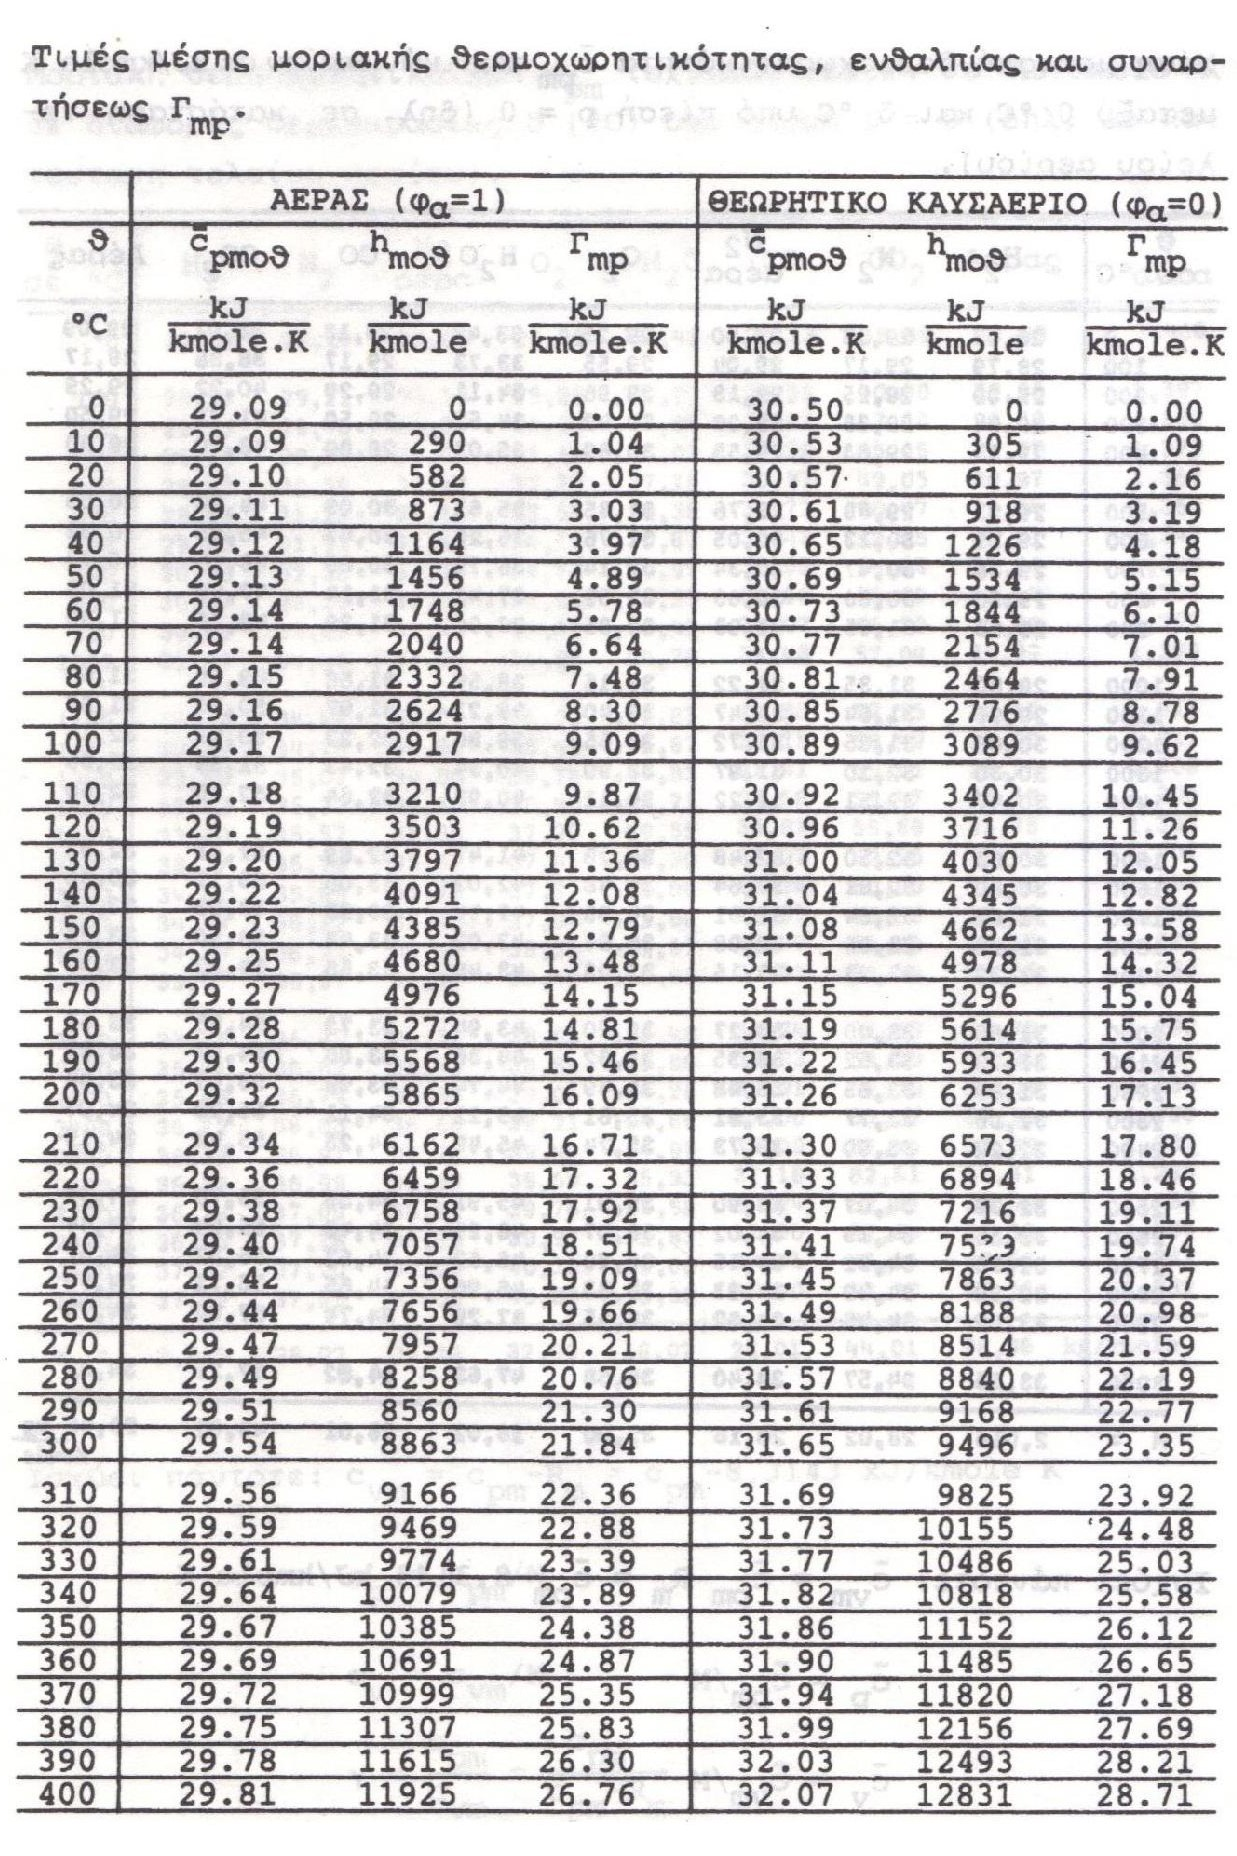
\includegraphics[width=1.2\textwidth]{tinywow_EIMEK-Pinakes_15484416_1.jpg}
    \end{subfigure}
    \hfill
    \begin{subfigure}[b]{.3\textwidth}
        \centering
        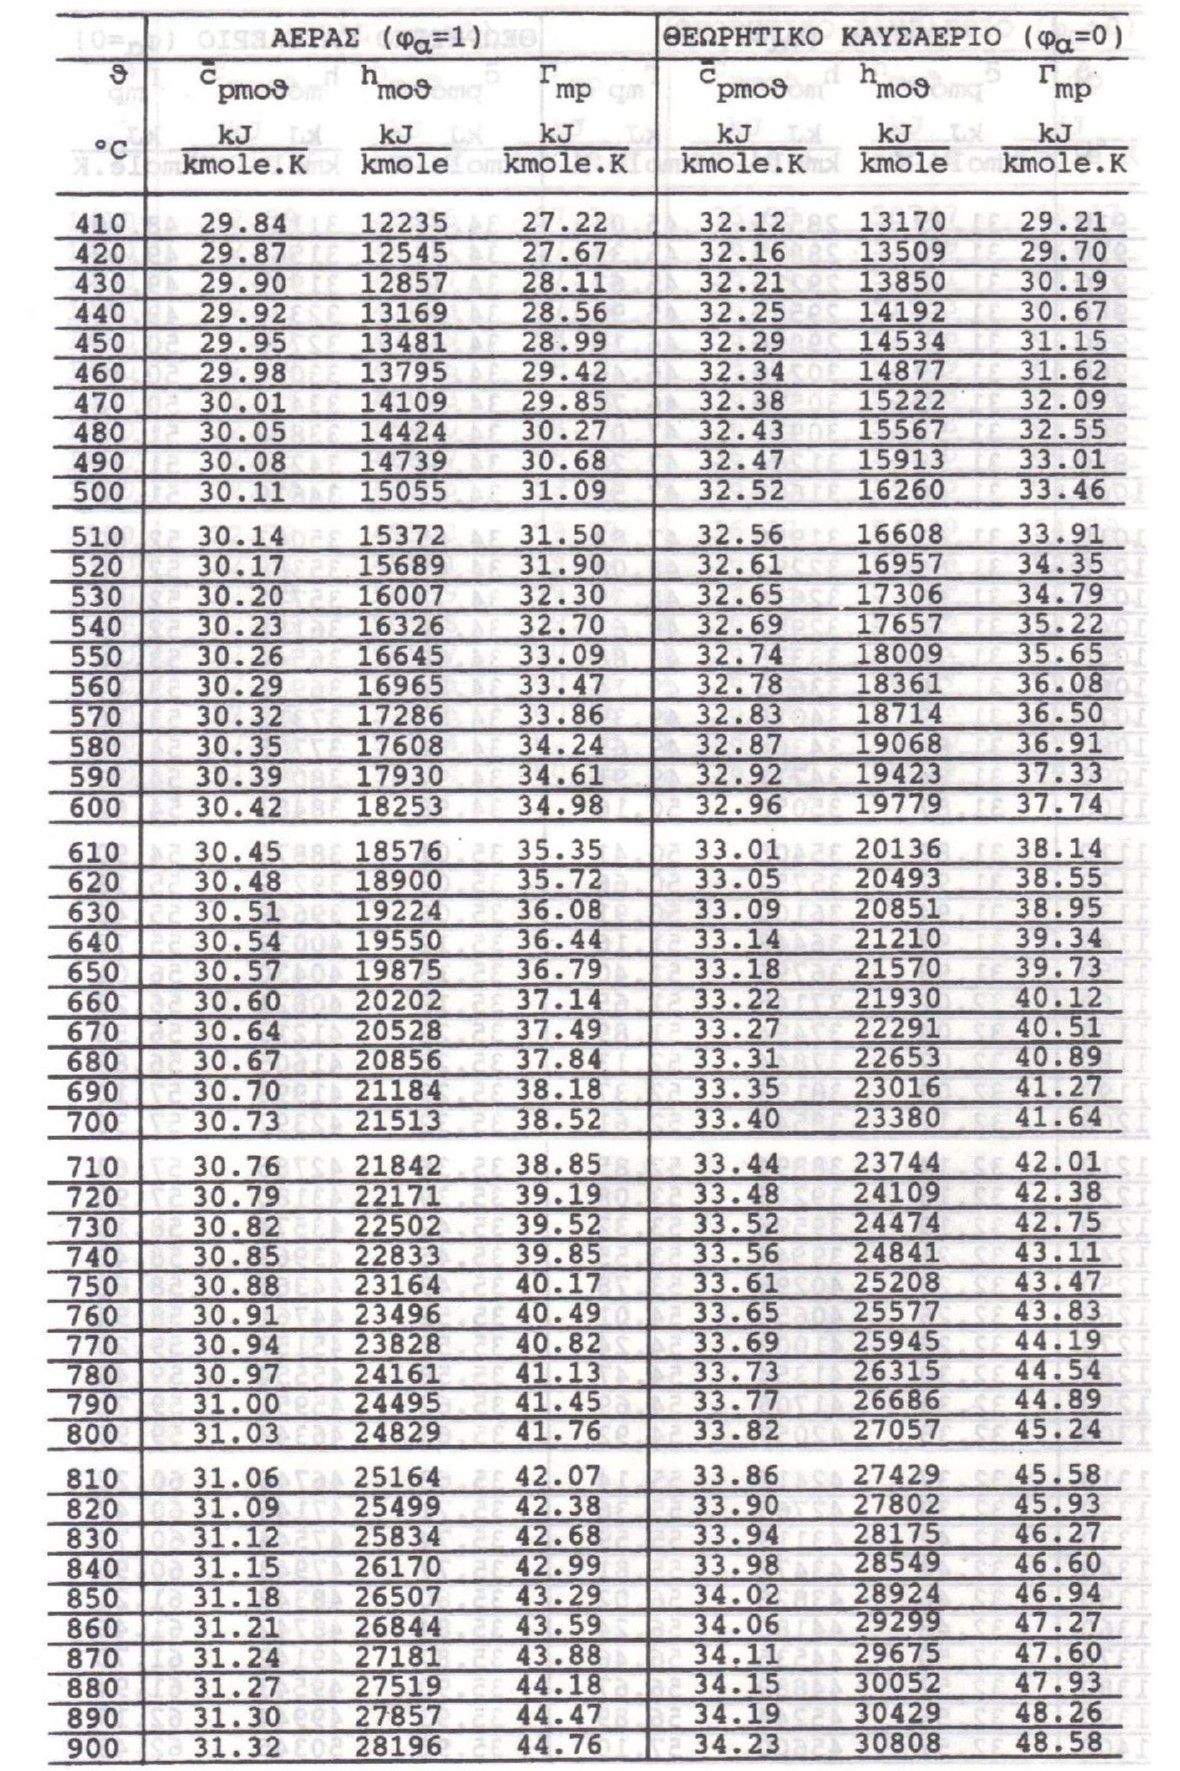
\includegraphics[width=1.2\textwidth]{tinywow_EIMEK-Pinakes_15484416_2.jpg}
    \end{subfigure}
    \hfill
    \begin{subfigure}[b]{.3\textwidth}
        \centering
        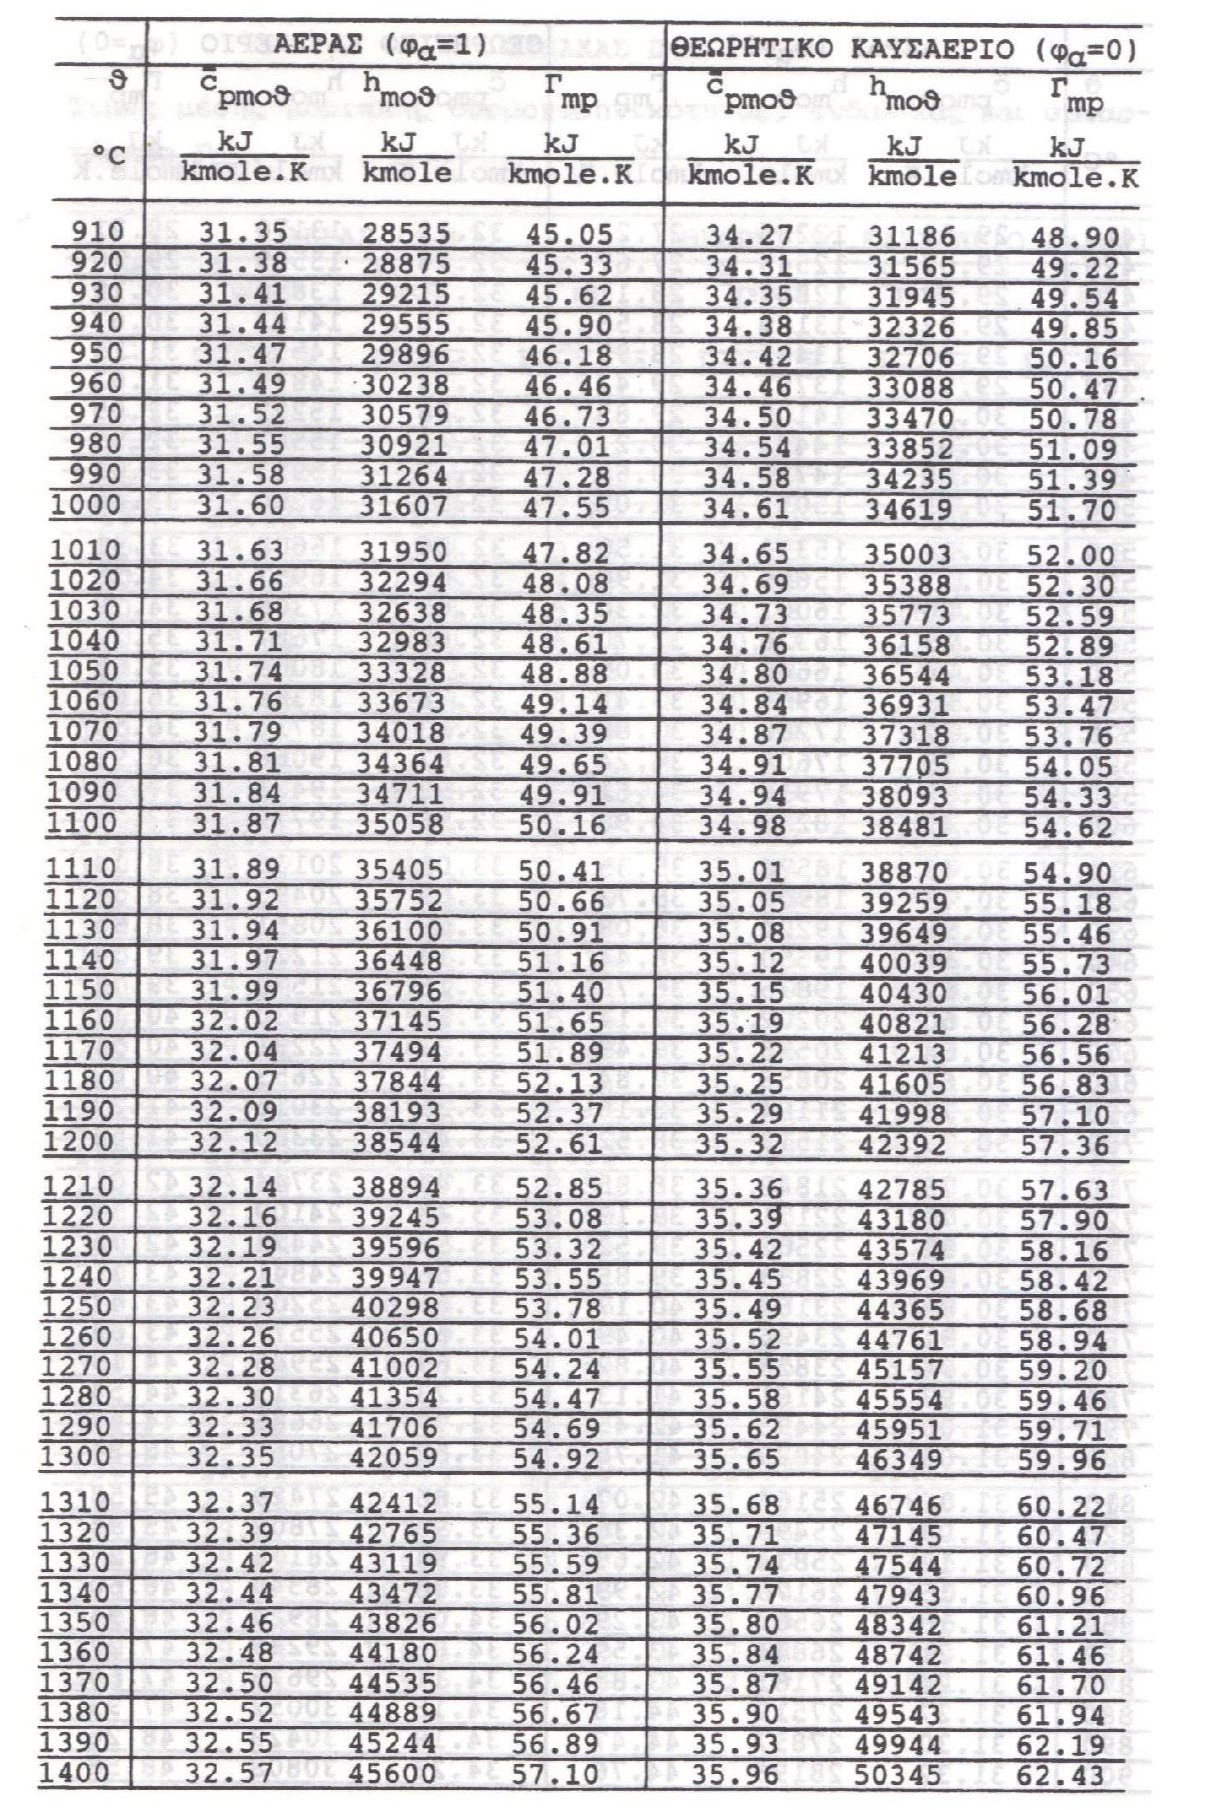
\includegraphics[width=1.2\textwidth]{tinywow_EIMEK-Pinakes_15484416_3.jpg}
    \end{subfigure}
    \caption{%Πίνακες ενθαλπίας
    Enthalpy tables}
    \label{fig:enthalpies}
\end{figure}

\begin{figure}[h]
    \centering
    \begin{subfigure}[b]{0.4\textwidth}
        \centering
        \includegraphics[width=1.2\textwidth]{tinywow_EIMEK-Typologio_15484510_1.jpg}
    \end{subfigure}
    \hfill
    \begin{subfigure}[b]{.4\textwidth}
        \centering
        \includegraphics[width=1.2\textwidth]{tinywow_EIMEK-Typologio_15484510_2.jpg}
    \end{subfigure}
    \caption{%Υποστηρηκτικές σημειώσεις
    Notes}
    \label{fig:ypost}
\end{figure}

\newpage
\section{%Μετρήσεις
Measurements}
%Οι μετρήσεις που έγιναν αφορούν 4 σημεία λειτουργίας. Το πρώτο με 2000 $rpm$ και 120 $Nm$, το δεύτερο με 2000 $rpm$ και 200 $Nm$, το τρίτο με 2300 $rpm$ και 80 $Nm$ και το τέταρτο με 2300 $rpm$ και 160 $Nm$. Οι μετρήσεις της \textbf{ΟΜΑΔΑΣ 12} με τις οποίες θα γίνουν και οι υπολογισμοί φαίνονται στον Πίνακα \ref{tab:metrhseis}.
The measurements were taken at four operating points: the first one at 2000 rpm and 120 Nm, the second one at 2000 $rpm$ and 200 $Nm$, the third one at 2300 $rpm$ and 80 $Nm$ and the fourth one at 2300 $rpm$ and 160 $Nm$. The measurements from \textbf{GROUP 12} which will be used for calculations, are shown in Table \ref{tab:metrhseis}.


%\selectlanguage{english}
\begin{table}[h]
    \centering
    \renewcommand{\arraystretch}{1.2}    
    \begin{tabular}{|c|c|c|c|c|c|c|c|c|c|c|c|}
    \hline
    \rowcolor{blue}
    \# & $Speed$ & $Torque$ & $Throttle$ & $T_{exh}$ & $T_{air}$ & $T_{w,in}$/$T_{w,out}$ & $Airflow$ & $INJ$ & $NO_x$ & $SOOT$ & $O_2$ \\
    \hline
    \rowcolor{gray}
    - & $rpm$ & $Nm$ & \% & $^\circ C$ & $^\circ C$ & $^\circ C$ & $Kg/h$ & $mg/str$ & $ppm$ & $mg/m^3$ & \% \\
    \hline
    1 & 2000 & 120 & 41 & 387 & 23.4 & 83/84 & 133 & 26.7 & 70 & 30 & 6.1 \\
    \hline
    2 & 2000 & 200 & 52.5 & 468 & 25.4 & 81/84 & 185 & 42.6 & 92 & 115 & 3.8 \\
    \hline
    3 & 2300 & 80 & 33.7 & 321 & 25.4 & 83/84 & 142 & 18.5 & 94 & 26 & 9.3 \\
    \hline
    4 & 2300 & 160 & 50.3 & 441 & 26.1 & 81/84 & 190 & 34.7 & 86 & 110 & 4.9 \\
    \hline
    \end{tabular}
    \caption{%Μετρήσεις ΟΜΑΔΑΣ 12
    GROUP 12 Measurements}
    \label{tab:metrhseis}
\end{table}

%\selectlanguage{greek}
Where:
\begin{enumerate}
    \item $\boldsymbol{T_{exh}}$ - Exhaust gas temperature
    \item $\boldsymbol{T_{air}}$ - Inlet air temperature
    \item $\boldsymbol{T_{w,in}}$ - Coolant (water) inlet temperature
    \item $\boldsymbol{T_{w,out}}$ - Coolant (water) outlet temperature
    \item $\boldsymbol{Airflow}$ - Mass flow rate of air at the intake for all four cylinders
    \item $\boldsymbol{INJ}$ - Fuel mass flow rate for one cylinder in one thermodynamic cycle
\end{enumerate}







\chapter{%Υπολογισμοί
Calculations}

\section{%Ερώτημα 1ο
Question 1}

%Για τους υπολογισμούς δημιουργήθηκε φύλλο εργασίας στο \selectlanguage{english}Excel \selectlanguage{greek}και χρησιμοποίηθηκε θεωρία από τις υποστηρηκτικές σημειώσεις του μαθήματος (Σχήμα \ref{fig:ypost}).\newlineΣτο πρώτο ερώτημα ζητέιτεαι να υπολογιστεί η παροχή μάζας του ψυκτικού, που στην περίπτωση αυτή είναι το νερό. Η παροχή μπορεί να υπολογιστεί μέσω του τύπου:\begin{equation}\label{eq:q.cool} \dot{Q}_{coolant}=\dot{m}_{coolant}\cdot c_{p_{coolant}}\cdot (T^{out}_{coolant}-T^{in}_{coolant})\quad (W)\end{equation}ωστόσο με την δοσμένη παραδοχή ότι η ισχύς του ψυκτικού είναι το 30\% της ισχύς του καυσίμου: \begin{equation} \label{eq:q.cool30} \dot{Q}_{coolant}=30\%\cdot \dot{Q}_{fuel}\end{equation}αρκεί η εύρεση της ισχύς του καυσίμου όπου αυτή υπολογίζεται ως: \begin{equation} \label{eq:q.fuel} \dot{Q}_{fuel}=\dot{m}_{fuel}\cdot H_u\quad (W\end{equation}
%όπου:\begin{itemize}\item $\boldsymbol{\dot{m}_{fuel}}$ η παροχή μάζας του καυσίμου \item $\boldsymbol{H_u}$ η θερμογόνως δύναμη του καυσίμου η οποία είναι γνωστή και δίνεται ως $H_u=42.5$ $MJ/kg$\end{itemize}Για τον υπολογισμό της παροχής του καυσίμου για κάθε σημείο λειτουργίας χρησιμοποιούνται οι μετρήσεις του $\boldsymbol{INJ}$, το όποιο δείχνει την παροχή μάζας του καυσίμου για 1 κύλινδρο σε 1 θερμοδυναμικό κύκλο, από τον Πίνακα \ref{tab:metrhseis}. Επίσης εφόσον ο κινητήρας είναι 4-χρονος ο ένας θερμοδυναμικός κύκλος προκύπτει σε 720$^\circ$, δηλαδή σε 2 στροφές ($1\:  stroke = 2 \: rotations$). Επομένως για τους 4 κυλίνδρους θα προκύψει: $$\dot{m}_{fuel}=4cylinders\cdot INJ(\frac{mg}{stroke})\cdot \frac{rotations}{min}<=>$$ $$\dot{m}_{fuel}=4cylinders\cdot INJ\frac{mg}{2\: rotations}\cdot \frac{rotations}{min}<=>$$$$\dot{m}_{fuel}=4cylinders\cdot INJ\cdot \frac{rpm}{2}\cdot \frac{10^{-6}kg}{60\:seconds}<=>$$\begin{equation} \label{eq:paroxhpsykt} \dot{m}_{fuel}=\frac{INJ\cdot rpm}{30000000}\quad (kg/s\end{equation}Επομένως χρησιμοποιώντας την εξίσωση \ref{eq:paroxhpsykt} για κάθε σημείο λειτουργίας μέσω του φύλλου εργασίας προκύπτουν οι τιμές της παροχής μάζας του καυσίμου οι οποίες φαίνονται στον Πίνακα \ref{tab:m.fuel}.\begin{table}[h] \centering \renewcommand{\arraystretch}{1.2}  \begin{tabular}{|c|c|c|} \hline \rowcolor{blue} $\#$ & $INJ$ & $\dot{m}_{fuel}$\\ \hline\rowcolor{gray}- & $mg/str$ & $kg/s$\\ \hline 1 & 26.7 & 0.00178\\ \hline 2 & 42.6 & 0.00284\\ \hline 3 & 18.5 & 0.001418333\\ \hline 4 & 34.7 & 0.002660333\\ \hline  \end{tabular} \caption{Τιμές παροχής μάζας καυσίμου για κάθε σημείο λειτουργίας} \label{tab:m.fuel}\end{table}\newpageΕφόσον οι τιμές της παροχής είναι γνωστές, μπορεί να υπολογιστεί η ισχύς του καυσίμου από την εξίσωση \ref{eq:q.fuel} για γνωστή $H_u=42500000$ $J/kg$. Μέσω αυτών των τιμών μπορεί επίσης να υπολογιστεί η ισχύς του ψυκτικού μέσω της σχέσης \ref{eq:q.cool30}. Τέλος υπολογίζεται η \textbf{παροχή μάζας του ψυκτικού} με γνωστή τη θερμοχωριτικότητα του ψυκτικού (νερό) $c_{p_{coolant}}=4180$ $J/kg\cdot K$ και με μια αναδιαμόρφωση της εξίσωσης \ref{eq:q.cool} ως εξής:$$\dot{m}_{coolant}=\frac{\dot{Q}_{coolant}}{c_{p_{coolant}}\cdot (T^{out}_{coolant}-T^{in}_{coolant})}\quad (kg/s)$$Με γνστές τις $T^{out}_{coolant}$ ($T_{w,in}$) και $T^{in}_{coolant}$ ($T_{w,out}$) για κάθε σημείο λειτουργίας από τον Πίνακα \ref{tab:metrhseis} οι παραπάνω τιμές υπολογίζονται με το φύλλο εργασίας και φαίνονται στον Πίνακα \ref{tab:finaltable1o}.\begin{table}[h] \centering\renewcommand{\arraystretch}{1.2} \begin{tabular}{|c|c|c|c|c|}\hline\rowcolor{blue}$\#$ & $\dot{m}_{fuel}$ & $\dot{Q}_{fuel}$ & $\dot{Q}_{coolant}$ & $\dot{m}_{coolant}$ \\\hline\rowcolor{gray}- & $kg/s$ & $W$ & $W$ & $kg/s$ \\ \hline 1 & 0.00178 & 75650 & 22695 & 5.43 \\\hline2 & 0.00284 & 120700 & 36210 & 2.89\\ \hline3 & 0.001418333 & 60279.17 & 18083.75 & 4.33\\\hline4 & 0.002660333 & 113064.17 & 33919.25 & 2.70 \\\hline \end{tabular}\caption{Τιμές παροχής μάζας ψυκτικού για κάθε σημείο λειτουργίας}\label{tab:finaltable1o}\end{table}Οι τιμές της παροχής μάζας του ψυκτικού φαίνονται και σε διάγραμμα για σταθερή περιστροφική ταχύτητα του κινητήρα στο Σχήμα \ref{fig:m./Torque}. Παρατηρείται ότι για \textbf{σταθερό} αριθμό στροφών $Ν$ και καθώς η ροπή του κινητήρα $Μ$ \textbf{αυξάνεται}, η παροχή μάζας του ψυκτικού $\dot{m}_{fuel}$ \textbf{μειώνεται}.\begin{figure}[!h]\centering 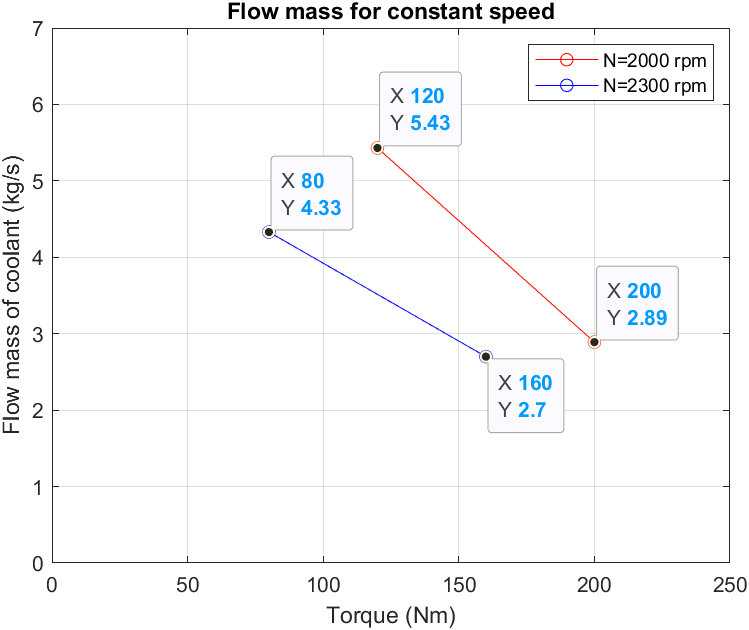
\includegraphics[width=.7\textwidth]{erwthma1.png}\caption{Παροχή μάζας ψυκτικού συναρτήσει της ροπής για σταθερές στροφές}\label{fig:m./Torque}\end{figure}


% Greek text with LaTeX code


For the calculations, an Excel spreadsheet was created and theory from the course's supporting notes was used (Figure \ref{fig:ypost}).\newline

In the first question, the mass flow rate of the coolant, which in this case is water, needs to be calculated. The flow can be calculated using the equation:

\begin{equation}
    \label{eq:q.cool}
    \dot{Q}_{coolant} = \dot{m}_{coolant} \cdot c_{p_{coolant}} \cdot (T^{out}_{coolant} - T^{in}_{coolant}) \quad (W)
\end{equation}

However, with the given assumption that the power of the coolant is 30\% of the power of the fuel:

\begin{equation}
    \label{eq:q.cool30}
    \dot{Q}_{coolant} = 30\% \cdot \dot{Q}_{fuel}
\end{equation}

It is sufficient to find the power of the fuel. That is calculated as:

\begin{equation}
    \label{eq:q.fuel}
    \dot{Q}_{fuel} = \dot{m}_{fuel} \cdot H_u \quad (W)
\end{equation}

where:
\begin{itemize}
    \item $\boldsymbol{\dot{m}_{fuel}}$ is the mass flow rate of the fuel
    \item $\boldsymbol{H_u}$ is the calorific value of the fuel, which is known and given as $H_u = 42.5$ $MJ/kg$
\end{itemize}

To calculate the fuel flow for each operating point, the measurements of $\boldsymbol{INJ}$, which shows the mass flow rate of the fuel for 1 cylinder in 1 thermodynamic cycle, from Table \ref{tab:metrhseis} are used. Also, since the engine is 4-stroke, one thermodynamic cycle corresponds to 720$^\circ$, which is equivalent to 2 rotations ($1\:stroke = 2\:rotations$). Therefore, for the 4 cylinders, it will be:

$$\dot{m}_{fuel} = 4\:cylinders \cdot INJ (\frac{mg}{stroke}) \cdot \frac{rotations}{min} <=>$$
$$\dot{m}_{fuel} = 4\:cylinders \cdot INJ \cdot \frac{mg}{2\:rotations} \cdot \frac{rotations}{min} <=>$$
$$\dot{m}_{fuel} = 4\:cylinders \cdot INJ \cdot \frac{rpm}{2} \cdot \frac{10^{-6}kg}{60\:seconds} <=>$$
\begin{equation}
    \label{eq:paroxhpsykt}
    \dot{m}_{fuel} = \frac{INJ \cdot rpm}{30000000} \quad (kg/s)
\end{equation}

Thus, by using Equation \ref{eq:paroxhpsykt}, the fuel mass flow rates for each operating point are calculated through the spreadsheet and shown in Table \ref{tab:m.fuel}.

% Table for fuel mass flow rates
\begin{table}[H]
    \centering
    \renewcommand{\arraystretch}{1.2} 
    \begin{tabular}{|c|c|c|}
    \hline
    \rowcolor{blue}
    $\#$ & $INJ$ & $\dot{m}_{fuel}$\\
    \hline
    \rowcolor{gray}
    - & $mg/str$ & $kg/s$\\
    \hline
    1 & 26.7 & 0.00178\\
    \hline
    2 & 42.6 & 0.00284\\
    \hline
    3 & 18.5 & 0.001418333\\
    \hline
    4 & 34.7 & 0.002660333\\
    \hline 
    \end{tabular}
    \caption{Fuel mass flow rates for each operating point}
    \label{tab:m.fuel}
\end{table}

Once the fuel mass flow rates are known, the power of the fuel can be calculated from Equation \ref{eq:q.fuel} using the known $H_u = 42500000$ $J/kg$. Through these values, the power of the coolant is also calculated using Equation \ref{eq:q.cool30}. Finally, the \textbf{mass flow rate of the coolant} is calculated with the known specific heat capacity of the coolant (water) $c_{p_{coolant}} = 4180$ $J/kg\cdot K$ and a rearrangement of Equation \ref{eq:q.cool} as follows:

$$\dot{m}_{coolant} = \frac{\dot{Q}_{coolant}}{c_{p_{coolant}} \cdot (T^{out}_{coolant} - T^{in}_{coolant})} \quad (kg/s)$$

Using the values of $T^{out}_{coolant}$ ($T_{w,in}$) and $T^{in}_{coolant}$ ($T_{w,out}$) for each operating point from Table \ref{tab:metrhseis}, these values are calculated through the spreadsheet and shown in Table \ref{tab:finaltable1o}.

% Table for coolant mass flow rates
\begin{table}[H]
    \centering
    \renewcommand{\arraystretch}{1.2} 
    \begin{tabular}{|c|c|c|c|c|}
    \hline
    \rowcolor{blue}
    $\#$ & $\dot{m}_{fuel}$ & $\dot{Q}_{fuel}$ & $\dot{Q}_{coolant}$ & $\dot{m}_{coolant}$ \\
    \hline
    \rowcolor{gray}
    - & $kg/s$ & $W$ & $W$ & $kg/s$ \\
    \hline
    1 & 0.00178 & 75650 & 22695 & 5.43 \\
    \hline
    2 & 0.00284 & 120700 & 36210 & 2.89\\
    \hline
    3 & 0.001418333 & 60279.17 & 18083.75 & 4.33\\
    \hline
    4 & 0.002660333 & 113064.17 & 33919.25 & 2.70 \\
    \hline 
    \end{tabular}
    \caption{Coolant mass flow rates for each operating point}
    \label{tab:finaltable1o}
\end{table}

The values of the coolant mass flow rates are also shown in a diagram for constant rotational speed of the engine in Figure \ref{fig:m./Torque}. It can be observed that for a \textbf{constant} number of revolutions $N$ and as the engine torque $M$ \textbf{increases}, the mass flow rate of the coolant $\dot{m}_{fuel}$ \textbf{decreases}.

\begin{figure}[!h]
    \centering
    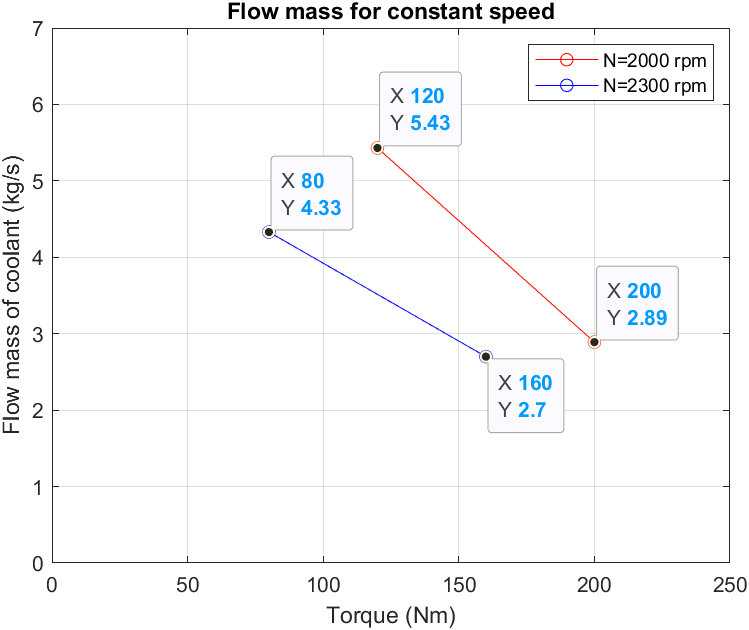
\includegraphics[width=.7\textwidth]{erwthma1.png}
    \caption{Coolant mass flow rate as a function of torque at constant RPM.}
    \label{fig:m./Torque}
\end{figure}






\newpage
\section{%Ερώτημα 2ο
Question 2}

%Το δεύτερο ερώτημα αφορά τον ενεργειακό ισολογισμό του κινητήρα καθώς και το ποσοστά προσδιδόμενης ενέργειας του κάθε όρου. Ο ενεργειακός ισολογισμός του κινητήρα υπολογίζεται από την σχέση:\begin{equation} \label{eq:energisol}\dot{Q}_{fuel}=P_e+\dot{Q}_{exhaust}+\dot{Q}_{coolant}+\dot{Q}_A\end{equation}όπου:\begin{itemize} \item $\boldsymbol{P_{e}}$ η πραγματική ισχύς του κινητήρα \item $\boldsymbol{\dot{Q}_A}$ οι άδηλες απώλειες \item $\boldsymbol{\dot{Q}_{exhaust}}$ η θερμική ισχύς του καυσαερίου \end{itemize}Η ισχύς του καυσίμου $\boldsymbol{\dot{Q}_{fuel}}$ και του ψυκτικού $\boldsymbol{\dot{Q}_{coolant}}$ φαίνονται στον Πίνακα \ref{tab:finaltable1o}. Επομένως χρειάζεται να υπολογιστούν μόνο η ισχύς του κινητήρα, η θερμική ισχύς και οι άδηλες απώλειες. Η $P_e$ υπολογίζεται ως εξής:$$P_e=M\cdot \omega<=>$$$$P_e=M\cdot \frac{2\pi \cdot N}{60}\quad (W)$$Με γνωστές την ροπή $Μ$ $(Nm)$ και την ταχύτητα $Ν$ $(rpm)$ προκύπτουν οι τιμές της $P_e$ $(W)$ για κάθε ένα από τα τέσσερα σημεία λειτουργίας στον Πίνακα \ref{tab:Pe}.\begin{table}[h]  \centering  \renewcommand{\arraystretch}{1.2}   \begin{tabular}{|c|c|c|c|} \hline \rowcolor{blue}  $\#$ & $N$ & $M$ & $P_{e}$\\ \hline \rowcolor{gray} - & $rpm$ & $Nm$ & $W$\\ \hline 1 & 2000 & 120 & 25132.74\\ \hline 2 & 2000 & 200 & 41887.90 \\ \hline 3 & 2300 & 80 & 19268.43\\ \hline 4 & 2300 & 160 & 38536.87\\ \hline  \end{tabular} \caption{Πραγματική ισχύς κινητήρα στα σημεία λειτουργίας} \label{tab:Pe}\end{table}Για τον υπολογισμό του $\dot{Q}_{exhaust}$ χρησιμοποιείται η σχέση:\begin{equation}  \label{eq:q.exh}  \dot{Q}_{exhaust}=\dot{m}_{exhaust}\cdot (h^{T_{exhaust}}_{exhaust}-h^{T_{ambient}}_{exhaust})\quad (W)\end{equation}όπου: \begin{itemize} \item $\boldsymbol{\dot{m}_{exhaust}}$ η παροχή μάζας του καυσαερίου \item $\boldsymbol{h^{T_{exhaust}}_{exhaust}}$ η ενθαλπία του καυσαερίου στη θερμοκρασία εξόδου από τον κινητήρα \item $\boldsymbol{h^{T_{ambient}}_{exhaust}}$ η ενθαλπία του καυσαερίου στη θερμοκρασία περιβάλλοντος\end{itemize}




The second question concerns the energy balance of the engine and the percentages of energy distribution for each term. The energy balance of the engine is described by the following equation:

\begin{equation}
    \label{eq:energisol}
    \dot{Q}_{fuel}=P_e+\dot{Q}_{exhaust}+\dot{Q}_{coolant}+\dot{Q}_A
\end{equation}

where:
\begin{itemize}
    \item $\boldsymbol{P_{e}}$ is the engine's true power.
    \item $\boldsymbol{\dot{Q}_A}$ represents the unaccounted losses.
    \item $\boldsymbol{\dot{Q}_{exhaust}}$ stands for the thermal power of the exhaust gas.
\end{itemize}

The power of the fuel $\boldsymbol{\dot{Q}_{fuel}}$ and the coolant $\boldsymbol{\dot{Q}_{coolant}}$ are shown in Table \ref{tab:finaltable1o}. Therefore, only the engine power, thermal power and unaccounted losses need to be calculated. $P_e$ is calculated as follows:

$$P_e=M\cdot \omega<=>$$
$$P_e=M\cdot \frac{2\pi \cdot N}{60}\quad (W)$$

With known values of torque $M$ $(Nm)$ and speed $N$ $(rpm)$, the values of $P_e$ $(W)$ are derived for each of the four operating points in Table \ref{tab:Pe}.

% Table for Pe
\begin{table}[h]
    \centering
    \renewcommand{\arraystretch}{1.2} 
    \begin{tabular}{|c|c|c|c|}
    \hline
    \rowcolor{blue}
    $\#$ & $N$ & $M$ & $P_{e}$\\
    \hline
    \rowcolor{gray}
    - & $rpm$ & $Nm$ & $W$\\
    \hline
    1 & 2000 & 120 & 25132.74\\
    \hline
    2 & 2000 & 200 & 41887.90 \\
    \hline
    3 & 2300 & 80 & 19268.43\\
    \hline
    4 & 2300 & 160 & 38536.87\\
    \hline 
    \end{tabular}
    \caption{Actual engine power at operating points}
    \label{tab:Pe}
\end{table}

To calculate $\dot{Q}_{exhaust}$, the following equation is used:

\begin{equation}
    \label{eq:q.exh}
    \dot{Q}_{exhaust}=\dot{m}_{exhaust}\cdot (h^{T_{exhaust}}_{exhaust}-h^{T_{ambient}}_{exhaust})\quad (W)
\end{equation}

where:

\begin{itemize}
    \item $\boldsymbol{\dot{m}_{exhaust}}$ is the mass flow rate of the exhaust gas.
    \item $\boldsymbol{h^{T_{exhaust}}_{exhaust}}$ is the enthalpy of the exhaust gas at the exit temperature from the engine.
    \item $\boldsymbol{h^{T_{ambient}}_{exhaust}}$ is the enthalpy of the exhaust gas at ambient temperature.
\end{itemize}





%Ισχύει η διατήρηση μάζας και συνεπώς:\begin{equation}\label{eq:m.exh}\dot{m}_{exhaust}=\dot{m}_{air}+\dot{m}_{fuel}\end{equation}Η παροχή μάζας του καυσίμου έχει υπολογιστεί στον Πίνακα \ref{tab:m.fuel} και η παροχή του αέρα από τις μετρήσεις του πειράμματος ανά ώρα ($Airflow$) στον Πίνακα \ref{tab:metrhseis}. Επομένως από τον τύπο \ref{eq:m.exh} υπολογίζεται η παροχή μάζας του καυσαερίου, αφού μετατραπεί από $kg/h$ σε $kg/s$ το $Airflow$, στον Πίνακα \ref{tab:m.exh}.\begin{table}[h] \centering \renewcommand{\arraystretch}{1.2}  \begin{tabular}{|c|c|c|c|} \hline \rowcolor{blue} $\#$ & $Airflow$ & $\dot{m}_{fuel}$ & $\dot{m}_{exhaust}$\\ \hline \rowcolor{gray} - & $kg/s$ & $kg/s$ & $kg/s$\\ \hline 1 & 0.036944444 & 0.00178 & 0.038724444\\ \hline 2 &  0.051388889 & 0.00284 & 0.054228889\\ \hline3 & 0.039444444 & 0.001418333 & 0.040862778\\\hline 4 & 0.052777778 & 0.002660333 & 0.055438111\\\hline  \end{tabular}\caption{Τιμές παροχής μάζας καυσαερίου για κάθε σημείο λειτουργίας} \label{tab:m.exh}\end{table}Η ενθαλπία του καυσαερίου υπολογίζεται κάθε φορά από την ενθαλπία του θεωρητικού καυσαερίου και του αέρα ως:\begin{equation}  \label{eq:h} h^T_{exhaust}=h^T_{air}\cdot \phi_{\alpha}+h^T_{theoretical}\cdot (1-\phi_{\alpha})\end{equation}Εδώ οι ενθαλπίες του αέρα και του θεωρητικού καυσίμου δίνονται από τους πίνακες ενθαλπίας (Σχήμα \ref{fig:enthalpies}) για τις διάφορες τιμές θερμοκρασίας. Οι θερμοκρασίες ενδιαφέροντος είναι οι $T_{exhaust}$ και $T_{air}$ από τον Πίνακα \ref{tab:metrhseis}. Με γραμμική παρεμβολή υπολογίζονται οι ζητούμενες ενθαλπίες στις τιμές αυτές ως εξής:\newlineΓια το πρώτο σημείο λειτουργίας ισχύει $Τ_{exhaust}=387^\circ C$ και $Τ_{air}=23.4^\circ C$. Με γραμμική παρεμβολή μεταξύ των τιμών $380-390^\circ C$ προκύπτουν οι $h^{T_{exhaust}}_{air}$ και $h^{T_{exhaust}}_{theoretical}$ ενώ με γραμμική παρεμβολή μεταξύ των τιμών $20-30^\circ C$ οι $h^{T_{ambient}}_{air}$ και $h^{T_{ambient}}_{theoretical}$. Αντίστοιχα υπολογίζονται οι υπόλοιπες ενθαλπίες. Αυτές φαίνονται στον Πίνακα \ref{tab:hair/htheo}.\newpage\begin{table}[!h]\centering \renewcommand{\arraystretch}{1.2}  \begin{tabular}{|c|c|c|c|c|} \hline \rowcolor{blue} $\#$ & $h^{T_{ambient}}_{air}$ & $h^{T_{exhaust}}_{air}$ & $h^{T_{ambient}}_{theoretical}$ & $h^{T_{exhaust}}_{theoretical}$\\ \hline \rowcolor{gray} - & $kJ/kmole$ & $kJ/kmole$ & $kJ/kmole$ & $kJ/kmole$\\ \hline 1 & 680.94 & 11522.6 & 715.38 & 12391.9\\ \hline 2 & 747.87 & 14046.2 & 785.99 & 15153\\\hline 3 & 747.87 & 9499.5 & 785.99 & 10188.1\\ \hline 4 & 759.51 & 13200.2 & 798.27 & 1426.2\\\hline \end{tabular} \caption{Ενθαλπίες αέρα και θεωρητικού καυσίμου στις θερμοκρασίες ενδιαφέροντος} \label{tab:hair/htheo\end{table}Έπειτα υπολογίζεται ο λόγος αέρα καυσίμου για κάθε σημείο λειτουργίας ως:$$\lambda_{\alpha}=\frac{\dot{m}_{air}}{\dot{m}_{fuel}}$$Από τις τιμές αυτές υπολογίζεται η περιεκτικότητα του καυσαερίου σε αέρα ως:$$\phi_{\alpha}=\frac{\lambda_{\alpha}-1}{\lambda_{\alpha}}$$Με γνωστό το μοριακό βάρος του καυσίμου και ίσο με $MB=28.98$ $kg/kmole$ και με μια απλή διαίρεση με τις τιμές στον Πίνακα \ref{tab:hair/htheo} υπολογίζονται οι ζητούμενες ενθαλπίες $\boldsymbol{h^{T_{ambient}}_{exhaust}}$ και $\boldsymbol{h^{T_{exhaust}}_{exhaust}}$ σε $\boldsymbol{kJ/kg}$ από τον τύπο \ref{eq:h}. Οι τιμές συνοψίζονται στον Πίνακα \ref{tab:l/phi/h}.\begin{table}[!h] \centering  \renewcommand{\arraystretch}{1.2}  \begin{tabular}{|c|c|c|c|c|}\hline \rowcolor{blue} $\#$ & $\lambda_{\alpha}$ & $\phi_{\alpha}$ & $h^{T_{ambient}}_{exhaust}$ $h^{T_{exhaust}}_{exhaust}$\\ \hline \rowcolor{gray} - & - & - & $kJ/kg$ & $kJ/kg$\\ \hline 1 &  20.75530587 & 0.951819549 & 399.0504923 & 23.55415234\\ \hline 2 & 18.09467919 & 0.944735135 & 486.7966581	& 25.87911307\\ \hline 3 & 27.81041911 & 0.964042254 &  328.6494308 & 25.85371668\\ \hline 4 & 19.83878378 & 0.949593684 & 457.2780152	& 26.27549168\\ \hline  \end{tabular} \caption{Ενθαλπίες καυσαερίου, λόγος αέρα και περιεκτικότητα σε αέρα του καυσίμου}\label{tab:l/phi/h}\end{table}

% Greek text with LaTeX code



The conservation of mass applies and therefore:

\begin{equation}
    \label{eq:m.exh}
    \dot{m}_{exhaust}=\dot{m}_{air}+\dot{m}_{fuel}
\end{equation}

The mass flow rate of fuel has been calculated in Table \ref{tab:m.fuel} and the mass flow rate of air is obtained from the experimental measurements per hour ($Airflow$) in Table \ref{tab:metrhseis}. Therefore, from equation \ref{eq:m.exh}, the mass flow rate of the exhaust gas is calculated after converting $Airflow$ from $kg/h$ to $kg/s$, as shown in Table \ref{tab:m.exh}.

% Table for mass flow rates
\begin{table}[h]
    \centering
    \renewcommand{\arraystretch}{1.2} 
    \begin{tabular}{|c|c|c|c|}
    \hline
    \rowcolor{blue}
    $\#$ & $Airflow$ & $\dot{m}_{fuel}$ & $\dot{m}_{exhaust}$\\
    \hline
    \rowcolor{gray}
    - & $kg/s$ & $kg/s$ & $kg/s$\\
    \hline
    1 & 0.036944444 & 0.00178 & 0.038724444\\
    \hline
    2 & 0.051388889 & 0.00284 & 0.054228889\\
    \hline
    3 & 0.039444444 & 0.001418333 & 0.040862778\\
    \hline
    4 & 0.052777778 & 0.002660333 & 0.055438111\\
    \hline 
    \end{tabular}
    \caption{Mass flow rate values for each operating point}
    \label{tab:m.exh}
\end{table}

The enthalpy of the exhaust gas is calculated each time using the enthalpy of theoretical fuel and air as follows:

\begin{equation}
    \label{eq:h}
    h^T_{exhaust}=h^T_{air}\cdot \phi_{\alpha}+h^T_{theoretical}\cdot (1-\phi_{\alpha})
\end{equation}

Here, the enthalpies of air and theoretical fuel are given by the enthalpy tables (Figure \ref{fig:enthalpies}) for various temperature values. The temperatures of interest are $T_{exhaust}$ and $T_{air}$ from Table \ref{tab:metrhseis}. Using linear interpolation between the values of $380-390^\circ C$ and $20-30^\circ C$, the values of $h^{T_{exhaust}}_{air}$, $h^{T_{exhaust}}_{theoretical}$, $h^{T_{ambient}}_{air}$, and $h^{T_{ambient}}_{theoretical}$ are obtained. The rest of the enthalpies are similarly calculated. These values are shown in Table \ref{tab:hair/htheo}.

% Table for enthalpy values
\begin{table}[!h]
    \centering
    \renewcommand{\arraystretch}{1.2} 
    \begin{tabular}{|c|c|c|c|c|}
    \hline
    \rowcolor{blue}
    $\#$ & $h^{T_{ambient}}_{air}$ & $h^{T_{exhaust}}_{air}$ & $h^{T_{ambient}}_{theoretical}$ & $h^{T_{exhaust}}_{theoretical}$\\
    \hline
    \rowcolor{gray}
    - & $kJ/kmole$ & $kJ/kmole$ & $kJ/kmole$ & $kJ/kmole$\\
    \hline
    1 & 680.94 & 11522.6 & 715.38 & 12391.9\\
    \hline
    2 & 747.87 & 14046.2 & 785.99 & 15153\\
    \hline
    3 & 747.87 & 9499.5 & 785.99 & 10188.1\\
    \hline
    4 & 759.51 & 13200.2 & 798.27 & 14226.2\\
    \hline 
    \end{tabular}
    \caption{Enthalpies of air and theoretical fuel at temperatures of interest}
    \label{tab:hair/htheo}
\end{table}

Next, the air-to-fuel ratio is calculated for each operating point as follows:

$$\lambda_{\alpha}=\frac{\dot{m}_{air}}{\dot{m}_{fuel}}$$

From these values, the air content of the fuel is determined as:

$$\phi_{\alpha}=\frac{\lambda_{\alpha}-1}{\lambda_{\alpha}}$$

With the known molecular weight of the fuel, which is $MB=28.98$ $kg/kmole$ and simple division by the values in Table \ref{tab:hair/htheo}, the required enthalpies $\boldsymbol{h^{T_{ambient}}_{exhaust}}$ and $\boldsymbol{h^{T_{exhaust}}_{exhaust}}$ in $\boldsymbol{kJ/kg}$ are calculated using equation \ref{eq:h}. These values are summarized in Table \ref{tab:l/phi/h}.

\begin{table}[!h] 
\centering  
\renewcommand{\arraystretch}{1.2}  
\begin{tabular}{|c|c|c|c|c|}
\hline 
\rowcolor{blue} $\#$ & $\lambda_{\alpha}$ & $\phi_{\alpha}$ & $h^{T_{ambient}}_{exhaust}$ & $h^{T_{exhaust}}_{exhaust}$\\ 
\hline 
\rowcolor{gray} - & - & - & $kJ/kg$ & $kJ/kg$\\ 
\hline 1 &  20.75530587 & 0.951819549 & 399.0504923 & 23.55415234\\ 
\hline 2 & 18.09467919 & 0.944735135 & 486.7966581	& 25.87911307\\ 
\hline 3 & 27.81041911 & 0.964042254 &  328.6494308 & 25.85371668\\ 
\hline 4 & 19.83878378 & 0.949593684 & 457.2780152	& 26.27549168\\ 
\hline  
\end{tabular} 
\caption{Combustion gas enthalpies, air-fuel ratio and air content of the fuel}
\label{tab:l/phi/h}
\end{table}




%Από τις τιμές των ενθαλπιών καυσαερίου (Πίνακας \ref{tab:l/phi/h}), της παροχής μάζας καυσαερίου (Πίνακας \ref{tab:m.exh}) και τον τύπο \ref{eq:q.exh} υπολογίζεται η \textbf{ισχύς του καυσαερίου} σε $kJ/s$. Πολλαπλασσιάζοντας με το $1000$ προκύπτει η τιμή σε $J/s=Watt$. Οι εν λόγω τιμές εμφανίζονται στον Πίνακα \ref{tab:q.exh}.\begin{table}[!h]\centering\renewcommand{\arraystretch}{1.2} \begin{tabular}{|c|c|}\hline\rowcolor{blue}$\#$ & $\dot{Q}_{exhaust}$\\\hline \rowcolor{gray} - & $W$\\ \hline 1 & 14540.89\\ \hline 2 & 24995.05\\ \hline3 & 12373.07\\ \hline 4 & 23893.97\\ \hline  \end{tabular \caption{Ισχύς καυσαερίου στα σημεία λειτουργίας} \label{tab:q.exh}\end{table}Πλέον μπορεί από τον τύπο \ref{eq:energisol} να υπολογιστούν και οι άδηλες απώλειες $\boldsymbol{\dot{Q}_A}$ εφόσον όλοι οι άλλοι όροι είναι γνωστοί. Όλες οι τιμές των όρων του ενεργειακού ισολογισμού καθώς και το \% της προσδιδόμενης ενέργειας για κάθε σημείο λειτουργίας δίνονται στον Πίνακα \ref{tab:finaltable2o}.\begin{table}[h]\centering\renewcommand{\arraystretch}{1.2}    \begin{tabular}{|c|c|c|c|c|c|c|c|c|c|c|}\hline\rowcolor{blue}$\#$ & \multicolumn{2}{| c |}{$\dot{Q}_{exhaust}$} & \multicolumn{2}{| c |}{$\dot{Q}_{coolant}$& \multicolumn{2}{| c |}{$P_{e}$} & \multicolumn{2}{| c |}{$\dot{Q}_{A}$} & \multicolumn{2}{| |}{$\dot{Q}_{fuel}$}\\\hline\rowcolor{gray}- & $W$ & \% & $W$ & \% & $W$ & \% & $W$ & \% & $W$ & \%\\\hline1 & 14540.89 & 19.22 & 22695 & 30 & 25132.74 & 33.22 & 13281.37 & 17.56 & 75650 & 100\\\hline2 & 24995.05 & 20.71 & 36210 & 30 & 41887.90 & 34.70 & 17607.05 & 14.59 & 120700 & 100\\\hline3 & 12373.07 & 20.53 & 18083.75 & 30 & 19268.43 & 31.97 & 10553.91 & 17.51 & 60279.17 & 100\\\hline4 & 23893.97 & 21.13 & 33919.25 & 30 & 38536.87 & 34.08 & 16714.08 & 14.78 & 113064.17 & 100\\\hline\end{tabular}\caption{Ενεργειακός ισολογισμός κινητήρα}\label{tab:finaltable2o}\end{table}Στο Σχήμα \ref{fig:isolfig} φαίνεται ο ενεργειακός ισολογισμός του κινητήρα για τις διάφορες τιμές της ροπής για σταθερό αριθμό στροφών.\begin{figure}[h]\centering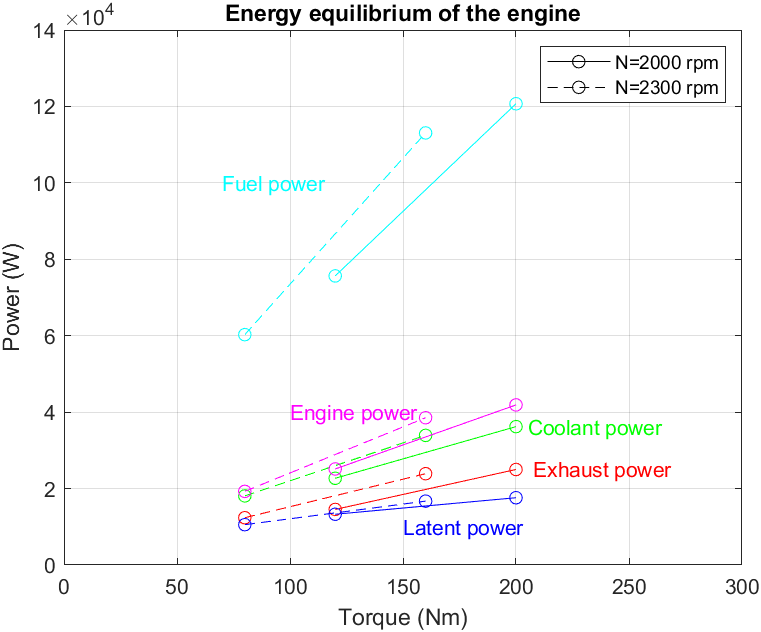
\includegraphics[width=0.7\textwidth]{erwthma2.png}\caption{%Ενεργειακός ισολογισμός κινητήραEngine energy equlibrium}\label{fig:isolfig}\end{figure}Παρατηρείται ότι για \textbf{σταθερό} αριθμό στροφών $N$ και καθώς η ροπή $Μ$ \textbf{αυξάνεται}, τα μεγέθη της ισχύος \textbf{αυξάνονται} επίσης.


% Greek text with LaTeX code


From the values of the exhaust gas enthalpies (Table \ref{tab:l/phi/h}), the mass flow rate of exhaust gas (Table \ref{tab:m.exh}) and equation \ref{eq:q.exh}, the \textbf{exhaust gas power} is calculated in $kJ/s$. Multiplying by 1000 the values are converted in $J/s = Watts$. These values are shown in Table \ref{tab:q.exh}.

% Table for exhaust gas power
\begin{table}[!h]
    \centering
    \renewcommand{\arraystretch}{1.2} 
    \begin{tabular}{|c|c|}
    \hline
    \rowcolor{blue}
    $\#$ & $\dot{Q}_{exhaust}$\\
    \hline
    \rowcolor{gray}
    - & $W$\\
    \hline
    1 & 14540.89\\
    \hline
    2 & 24995.05\\
    \hline
    3 & 12373.07\\
    \hline
    4 & 23893.97\\
    \hline 
    \end{tabular}
    \caption{Exhaust gas power at operating points}
    \label{tab:q.exh}
\end{table}

Now, from equation \ref{eq:energisol}, the \textbf{latent power} $\boldsymbol{\dot{Q}_A}$ can be calculated since all the other terms are known. All the values of the terms in the energy balance, as well as the \% of the provided energy for each operating point, are given in Table \ref{tab:finaltable2o}.

% Table for energy balance
\begin{table}[h]
    \centering
    \renewcommand{\arraystretch}{1.2}    
    \begin{tabular}{|c|c|c|c|c|c|c|c|c|c|c|}
    \hline
    \rowcolor{blue}
    $\#$ & \multicolumn{2}{| c |}{$\dot{Q}_{exhaust}$} & \multicolumn{2}{| c |}{$\dot{Q}_{coolant}$} & \multicolumn{2}{| c |}{$P_{e}$} & \multicolumn{2}{| c |}{$\dot{Q}_{A}$} & \multicolumn{2}{| c |}{$\dot{Q}_{fuel}$}\\
    \hline
    \rowcolor{gray}
    - & $W$ & \% & $W$ & \% & $W$ & \% & $W$ & \% & $W$ & \%\\
    \hline
    1 & 14540.89 & 19.22 & 22695 & 30 & 25132.74 & 33.22 & 13281.37 & 17.56 & 75650 & 100\\
    \hline
    2 & 24995.05 & 20.71 & 36210 & 30 & 41887.90 & 34.70 & 17607.05 & 14.59 & 120700 & 100\\
    \hline
    3 & 12373.07 & 20.53 & 18083.75 & 30 & 19268.43 & 31.97 & 10553.91 & 17.51 & 60279.17 & 100\\
    \hline
    4 & 23893.97 & 21.13 & 33919.25 & 30 & 38536.87 & 34.08 & 16714.08 & 14.78 & 113064.17 & 100\\
    \hline
    \end{tabular}
    \caption{Engine energy balance}
    \label{tab:finaltable2o}
\end{table}

In Figure \ref{fig:isolfig}, the energy balance of the engine for various torque values for constant speed $N$ is shown.

% Figure for energy balance
\begin{figure}[h]
\centering
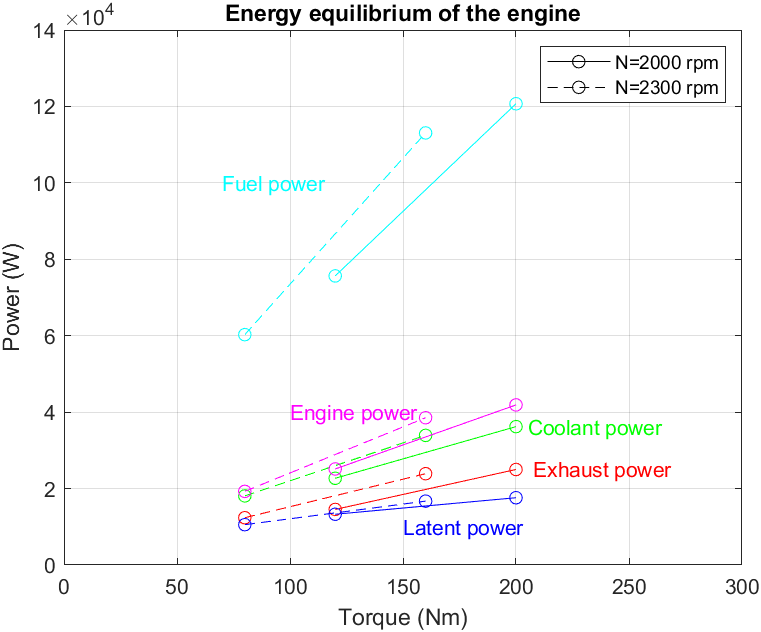
\includegraphics[width=0.7\textwidth]{erwthma2.png}
\caption{%Ενεργειακός ισολογισμός κινητήρα
Engine energy equilibrium}
\label{fig:isolfig}
\end{figure}

It is observed that for \textbf{constant} speed $N$ and as the torque $M$ \textbf{increases}, the power values \textbf{also increase}.








\section{%Ερώτημα 3ο
Question 3}

%Στο ερώτημα τρία ζητείται η ειδική κατανάλωση του καυσίμου (\selectlanguage{english}SFC)\selectlanguage{greek} για κάθε σημείο λειτουργίας. Έχοντας συγκεντρώσει δεδομένα από τα προηγούμενα ερωτήματα αυτή υπολογίζεται ως:

%$$specific\; fuel\; consumption\; (SFC)=\frac{rate\; of\; fuel\; consumption}{energy\; produced\; by\; the\; engine}$$

%Αυτό μεταφράζεται ως:

%\begin{equation}
%    \label{eq:SFC}
%    SFC=\frac{\dot{m}_{fuel}}{P_e}\quad (gr/kWh)
%\end{equation}

%όπου η $\boldsymbol{\dot{m}_{fuel}}$ σε $\boldsymbol{gr/h}$ και η $\boldsymbol{P_e}$ σε %$\boldsymbol{kW}$. Για αυτά ισχύει ότι:\newline

%\begin{equation}
%    \label{eq:metatropes}
%    \dot{m}_{fuel}\:(gr/h)=\dot{m}_{fuel}\: (kg/s)\cdot 3.6\times 10^6 \quad \&\quad P_e\: %(kW)=1000\cdot P_e\: (W)
%\end{equation}
%\newpage
%Επίσης για τον βαθμό απόδοσης ισχύει ότι:

%$$\eta=\frac{work\: done\: by\: the\: engine}{heat\: absorbed\: by\: the\: engine}<=>$$

%\begin{equation}
 %   \label{eq:eta}
 %   \eta=\frac{P_e}{\dot{Q}_{fuel}}
%\end{equation}

%Επομένως εύκολα μπορεί να προκύψει η σχέση του βαθμού απόδοσης με την ειδική κατανάλωση καυσίμου ως:

%$$\eta=\frac{P_e}{\dot{Q}_{fuel}}<=>$$
%$$\eta=\frac{P_e}{\dot{m}_{fuel}\cdot H_u}<=>$$

%\begin{equation}
%    \label{eq:sfc/eta}
%    \eta=\frac{1}{SFC\cdot H_u}
%\end{equation}

%Οι τιμές του βαθμού απόδοσης και της ειδικής κατανάλωσης καυσίμου προκύπτουν από τους Πίνακες \ref{tab:finaltable1o} και \ref{tab:Pe} καθώς και από τους τύπους \ref{eq:SFC}, \ref{eq:metatropes} και \ref{eq:eta} και φαίνονται στον Πίνακα \ref{tab:finaltable3o},

%\begin{table}[!h]
%    \centering
%    \renewcommand{\arraystretch}{1.2} 
%    \begin{tabular}{|c|c|c|c|c|c|}
%    \hline
%    \rowcolor{blue}
%    $\#$ & $\dot{m}_{fuel}$ & $P_e$ & $SFC$ & $\eta$ & $\eta$\\
%    \hline
%    \rowcolor{gray}
%    - & $gr/h$ & $kW$ & $gr/kWh$ & - & \%\\
%    \hline
%    1 & 6408 & 25.13 & 254.97 & 0.3322 & 33.22\\
%    \hline
%    2 & 10224 & 41.89 & 244.08 & 0.3470 & 34.70\\
%    \hline
%    3 & 5106 & 19.27 & 264.99 & 0.3197 & 31.97\\
 %   \hline
%    4 & 9577.2 & 38.54 & 248.52	& 0.3408 & 34.08\\
%    \hline 
%    \end{tabular}
%    \caption{Ειδική κατανάλωση καυσίμου και βαθμός απόδοσης}
%    \label{tab:finaltable3o}
%\end{table}

%Στο Σχήμα \ref{fig:SFC/eta} φαίνονται η ειδική κατανάλωση καυσίμου και ο βαθμός απόδοσης συναρτήσει %της ροπής του κινητήρα για σταθερό αριθμό στροφών. Παρατηρείται ότι για \textbf{σταθερό} αριθμό %στροφών $N$ και καθώς η ροπή $M$ \textbf{αυξάνεται}, η ειδική κατανάλωση καυσίμου $SFC$ %\textbf{μειώνεται} ενώ ο βαθμός απόδοσης $\eta$ \textbf{αυξάνεται}.

%\begin{figure}[!h]
%    \centering
%    \begin{subfigure}[b]{.49\textwidth}
%        \centering
%        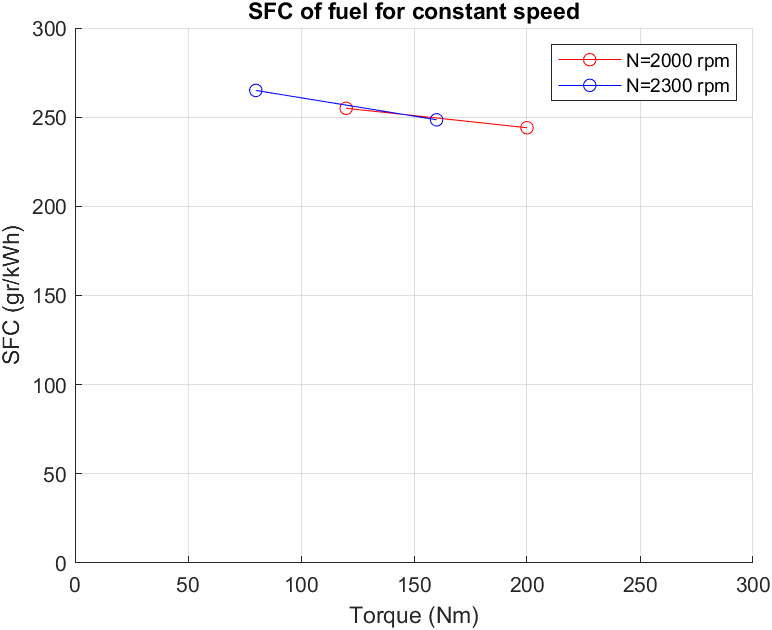
\includegraphics[width=\textwidth]{erwthma3b.png}
%    \end{subfigure}
%    \hfill
%    \begin{subfigure}[b]{.49\textwidth}
%        \centering
%        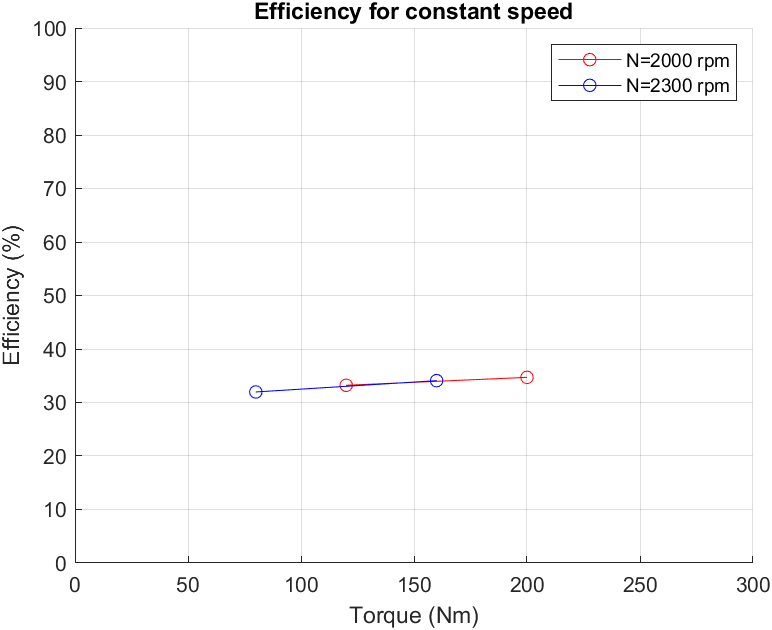
\includegraphics[width=\textwidth]{erwthma3a.png}
%    \end{subfigure}
%    \caption{Ειδική κατανάλωση καυσίμου και βαθμός απόδοσης για σταθερό αριθμό στροφών}
%    \label{fig:SFC/eta}
%\end{figure}
%\newpage




In question three, the specific fuel consumption (SFC) for each operating point is requested. Having gathered data from the previous questions, it is calculated as:

$$specific\; fuel\; consumption\; (SFC)=\frac{rate\; of\; fuel\; consumption}{energy\; produced\; by\; the\; engine}$$

This translates to:

\begin{equation}
    \label{eq:SFC}
    SFC=\frac{\dot{m}_{fuel}}{P_e}\quad (gr/kWh)
\end{equation}

where $\boldsymbol{\dot{m}_{fuel}}$ is in $\boldsymbol{gr/h}$ and $\boldsymbol{P_e}$ is in $\boldsymbol{kW}$. For these, it holds that:\newline

\begin{equation}
    \label{eq:metatropes}
    \dot{m}_{fuel}\:(gr/h)=\dot{m}_{fuel}\: (kg/s)\cdot 3.6\times 10^6 \quad \&\quad P_e\: (kW)=1000\cdot P_e\: (W)
\end{equation}
\newpage
Also, for the efficiency, it holds that:

$$\eta=\frac{work\: done\: by\: the\: engine}{heat\: absorbed\: by\: the\: engine}<=>$$

\begin{equation}
    \label{eq:eta}
    \eta=\frac{P_e}{\dot{Q}_{fuel}}
\end{equation}

Therefore, the relationship between efficiency and specific fuel consumption can be easily derived as:

$$\eta=\frac{P_e}{\dot{Q}_{fuel}}<=>$$
$$\eta=\frac{P_e}{\dot{m}_{fuel}\cdot H_u}<=>$$

\begin{equation}
    \label{eq:sfc/eta}
    \eta=\frac{1}{SFC\cdot H_u}
\end{equation}

The values of efficiency and specific fuel consumption are obtained from Tables \ref{tab:finaltable1o} and \ref{tab:Pe}, as well as from equations \ref{eq:SFC}, \ref{eq:metatropes}, and \ref{eq:eta} and are shown in Table \ref{tab:finaltable3o}:

\begin{table}[!h]
    \centering
    \renewcommand{\arraystretch}{1.2} 
    \begin{tabular}{|c|c|c|c|c|c|}
    \hline
    \rowcolor{blue}
    $\#$ & $\dot{m}_{fuel}$ & $P_e$ & $SFC$ & $\eta$ & $\eta$\\
    \hline
    \rowcolor{gray}
    - & $gr/h$ & $kW$ & $gr/kWh$ & - & \%\\
    \hline
    1 & 6408 & 25.13 & 254.97 & 0.3322 & 33.22\\
    \hline
    2 & 10224 & 41.89 & 244.08 & 0.3470 & 34.70\\
    \hline
    3 & 5106 & 19.27 & 264.99 & 0.3197 & 31.97\\
    \hline
    4 & 9577.2 & 38.54 & 248.52 & 0.3408 & 34.08\\
    \hline 
    \end{tabular}
    \caption{Specific fuel consumption and efficiency}
    \label{tab:finaltable3o}
\end{table}

In Figure \ref{fig:SFC/eta}, the specific fuel consumption and efficiency are shown as a function of engine torque for constant engine speed. It is observed that for \textbf{constant} engine speed $N$ and as the torque $M$ \textbf{increases}, the specific fuel consumption $SFC$ \textbf{decreases}, while efficiency $\eta$ slightly \textbf{increases}.

\begin{figure}[!h]
    \centering
    \begin{subfigure}[b]{.49\textwidth}
        \centering
        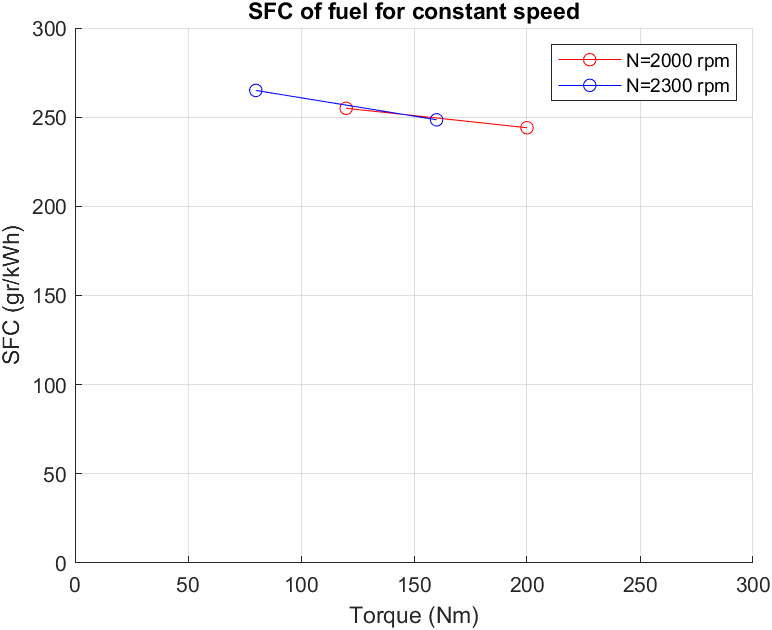
\includegraphics[width=\textwidth]{erwthma3b.png}
    \end{subfigure}
    \hfill
    \begin{subfigure}[b]{.49\textwidth}
        \centering
        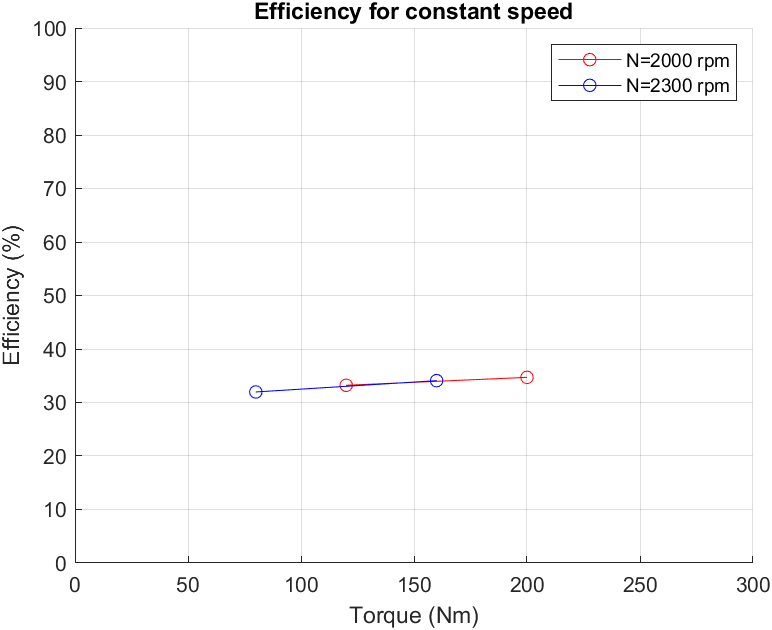
\includegraphics[width=\textwidth]{erwthma3a.png}
    \end{subfigure}
    \caption{Specific fuel consumption and efficiency for constant RPM.}
    \label{fig:SFC/eta}
\end{figure}






%\section{Ερώτημα 4ο}

%Στο τέταρτο ερώτημα ζητείται ο λόγος ισοδυναμίας αέρα-καυσίμου (\selectlanguage{english}AFR)\selectlanguage{greek} για κάθε σημείο λειτουργίας. Ο λόγος αυτός είναι ίσος με:
 
 %\begin{equation}
 %    \label{eq:AFR}
 %    AFR=\frac{\lambda_{real}}{\lambda_{stoich}}
% \end{equation}

%Το $\lambda_{stoich}$ είναι γνωστό και δοσμένο ως $\boldsymbol{\lambda_{stoich}=14.5}$ ενώ το $\lambda_{real}=\lambda_a$ το οποίο έχει υπολογιστεί στον Πίνακα \ref{tab:l/phi/h}. Επομένως οι τιμές του $AFR$ μπορούν να υπολογιστούν εύκολα από τον τύπο \ref{eq:AFR}. Οι τιμές αυτές δίνονται στον Πίνακα \ref{tab:AFR}.

%\begin{table}[h]
%    \centering
 %   \renewcommand{\arraystretch}{1.2} 
 %   \begin{tabular}{|c|c|c|c|}
%    \hline
%    \rowcolor{blue}
%    $\#$ & $\lambda_a$ & $AFR$\\\hline\rowcolor{gray}- & - & -\\\hline1 & 20.7553 & 1.4314\\\hline2 & 18.0947 & 1.2479\\\hline3 & 27.8104 & 1.9180\\\hline4 & 19.8388 & 1.3682\\\hline \end{tabular}\caption{Τιμές λόγου ισοδυναμίας αέρα καυσίμου για τα σημεία λειτουργίας} \label{tab:AFR}\end{table}Στο Σχήμα \ref{fig:AFR} φαίνονται οι τιμές του λόγου ισοδυναμίας αέρα-καυσίμου στα σημεία λειτουργίας. Παρατηρείται ότι για \textbf{σταθερό} αριθμό στροφών $N$ και καθώς η ροπή $M$ \textbf{αυξάνεται}, ο λόγος ισοδυναμίας αέρα-καυσίμου $AFR$ \textbf{μειώνεται}.\begin{figure}[h]\centering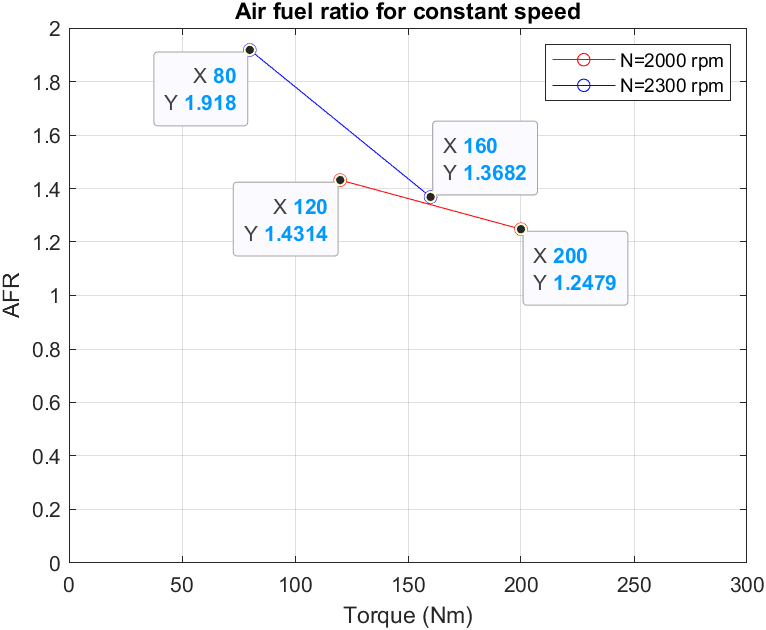
\includegraphics[width=0.7\textwidth]{erwthma4.png}\caption{Λόγος ισοδυναμίας αέρα-καυσίμου για σταθερό αριθμό στροφών}\label{fig:AFR}\end{figure}

\newpage
\section{Question 4}

In the fourth question, the air-fuel equivalence ratio (AFR) is requested for each operating point. This ratio is defined as:

\begin{equation}
    \label{eq:AFR}
    AFR=\frac{\lambda_{real}}{\lambda_{stoich}}
\end{equation}

Where $\lambda_{stoich}$ is known and given as $\boldsymbol{\lambda_{stoich}=14.5}$, while $\lambda_{real}=\lambda_a$, which has been calculated and is presented in Table \ref{tab:l/phi/h}. Therefore, the values of $AFR$ can be easily computed using equation \ref{eq:AFR}. These values are provided in Table \ref{tab:AFR}.

\begin{table}[h]
    \centering
    \renewcommand{\arraystretch}{1.2} 
    \begin{tabular}{|c|c|c|}
    \hline
    \rowcolor{blue}
    $\#$ & $\lambda_a$ & $AFR$\\
    \hline
    \rowcolor{gray}
    - & - & -\\
    \hline
    1 & 20.7553 & 1.4314\\
    \hline
    2 & 18.0947 & 1.2479\\
    \hline
    3 & 27.8104 & 1.9180\\
    \hline
    4 & 19.8388 & 1.3682\\
    \hline 
    \end{tabular}
    \caption{Air-Fuel Equivalence Ratio Values for Operating Points}
    \label{tab:AFR}
\end{table}

In Figure \ref{fig:AFR}, the values of the air-fuel equivalence ratio are plotted for the operating points. It is observed that for a \textbf{constant} engine speed $N$ and as the torque $M$ \textbf{increases}, the air-fuel equivalence ratio $AFR$ \textbf{decreases}.

\begin{figure}[h]\centering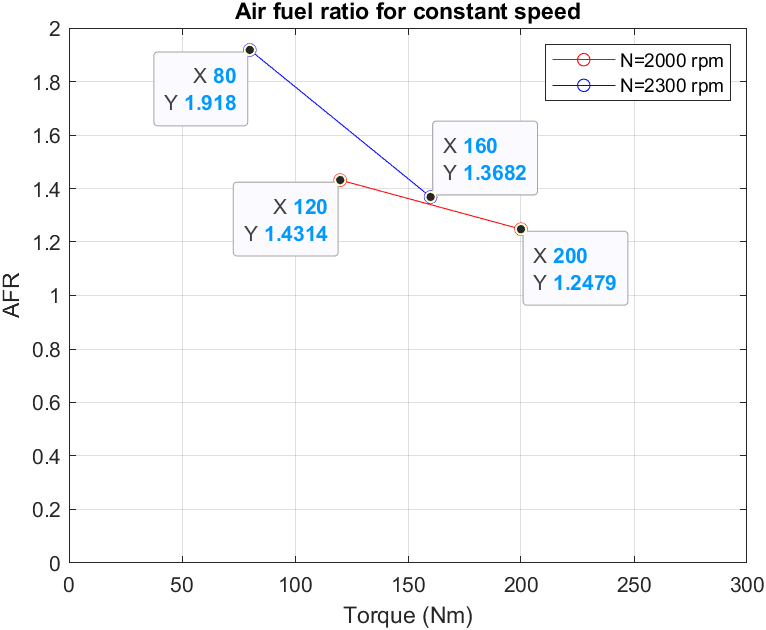
\includegraphics[width=0.7\textwidth]{erwthma4.png}\caption{Air-fuel equivalence ratio for constant RPM.}\label{fig:AFR}\end{figure}







\newpage
%\section{Ερώτημα 5ο}Στο πέμπτο και τελευταίο ερώτημα ζητούνται οι ειδικές εκπομπές $NO_x$ και $SOOT$. Αντίστοιχα με την ειδική κατανάλωση καυσίμου (Εξίσωση \ref{eq:SFC}), οι ειδικές εκπομπές μπορούν να οριστούν ως:\begin{equation}\label{eq:SNOxE}SNO_xE=\frac{\dot{m}_{NO_x}}{P_e}\quad (mg/kWh)\end{equation}\begin{equation}\label{eq:SSOOTE}SSOOTE=\frac{\dot{m}_{SOOT}}{P_e}\quad (mg/kWh)\end{equation}Αρκεί λοιπόν να υπολογιστούν οι παροχές μάζας των ρύπων. Με βάση τα δεδομένα του Πίνακα \ref{tab:metrhseis} προκύπτει η πυκνότητα του $NO_x$ σε $ppm$. Για την μετατροπη σε $mg/h$ ακολουθείται η εξής διαδικασία:$$NOx\:(ppm)=\frac{n_{solute}\: (mol)}{n_{solution}\: (mol)}\times 10^6<=>$$$$NOx\:(ppm)=\frac{\dot{n}_{solute}\: (mol/s)}{\dot{n}_{solution}\: (mol/s)}\times 10^6<=>$$$$NOx\:(ppm)=\frac{\dot{n}_{NO_x}\: (mol/s)}{\dot{n}_{exhaust}\: (mol/s)}\times 10^6<=>$$$$NOx\:(ppm)=\frac{\frac{\dot{m}_{NO_x}\: (kg/s)}{MB_{NO_x}\: (kg/mol)}}{\frac{\dot{m}_{exhaust}\: (kg/s)}{MB_{exhaust}\: (kg/mol)}}\times 10^6<=>$$\begin{equation}\label{eq:m.NOx}\dot{m}_{NO_x}\: (kg/s)=\frac{\dot{m}_{exhaust}\: (kg/s)\cdot NO_x\:(ppm)\cdot MB_{NO_x}\: (kg/mol)}{MB_{exhaust}\: (kg/mol)}\times 10^{-6} \end{equation}\begin{equation}\label{eq:m.NOx2}\dot{m}_{NO_x}\: (mg/h)= \dot{m}_{NO_x}\: (kg/s) \cdot 36\times 10^8\end{equation}Οντας γνωστές οι τιμές των μοριακών βαρών και δοσμένες ως $MB_{NO_x}=0.0460055\: kg/mol$ $MB_{exhaust}=0.02898\: kg/mol$, μέσω των σχέσεων \ref{eq:m.NOx}, \ref{eq:m.NOx2} και των τιμών από τον Πίνακα \ref{tab:m.exh} υπολογίζονται στον Πίνακα \ref{tab:m.NO_x} οι τιμές της παροχής μάζας του $NO_x$.\begin{table}[h]\centering \renewcommand{\arraystretch}{1.2}  \begin{tabular}{|c|c|c|c|}  \hline \rowcolor{blue} $\#$ & $NO_x$ & $\dot{m}_{NO_x}$ & $\dot{m}_{NO_x}$\\ \hline \rowcolor{gray}  - & $ppm$ & $\times 10^{-6}\: kg/s$ & $mg/h$\\  \hline  1 & 70 & 4.303 & 15491.63\\  \hline  2 & 92 & 7.920 & 28512.31\\  \hline  3 & 94 & 6.098 & 21951.77\\  \hline  4 & 86 & 7.569 & 27247.13\\  \hline   \end{tabular}  \caption{Τιμές παροχής μάζας $NO_x$ για κάθε σημείο λειτουργίας}  \label{tab:m.NO_x\end{table}Επομένως μέσω του τύπου \ref{eq:SNOxE}, από τις τιμές της παροχής μάζας του $NO_x$ ($mg/h$) και από τις τιμές της ισχύος του Πίνακα \ref{tab:finaltable3o} υπολογίζεται η ζητούμενη ειδική εκπομπή. Οι τιμές φαίνονται στον Πίνακα \ref{tab:finaltable5oa}.\begin{table}[!h]\centering \renewcommand{\arraystretch}{1.2}  \begin{tabular}{|c|c|}  \hline  \rowcolor{blue}  $\#$ & $SNO_xE$\\  \hline  \rowcolor{gray}  - & $mg/kWh$\\  \hline  1 & 616.39\\  \hline 2 & 680.68\\  \hline  3 & 1139.26\\  \hline  4 & 707.04\\  \hline   \end{tabular}  \caption{Ειδική εκπομπή $NO_x$ στα σημεία λειτουργίας} \label{tab:finaltable5oa}\end{table}Για τον υπολογισμό της ειδικής εκπομπής  $SOOT$ πρέπει να προσδιοριστεί πάλι η παροχή μάζας του. Είναι γνωστό από την Θερμοδυναμική ότι ένα μείγμα αεριών μπορεί να θεωρηθεί ως ένα νέο ιδανικό αερίο. Εντούτοις το καυσαέριο μείγμα μπορεί να θεωρηθεί ιδανικό αέριο για το οποίο η Καταστατική Εξίσωση των Ιδανικών Αερίων γράφεται ως:$$P\cdot V=n\cdot R\cdot T<=>$$$$P=\frac{\rho_{exhaust}}{MB_{exhaust}}\cdot R\cdot T_{exhaust}<=>$$\rho_{exhaust}=\frac{P\cdot MB_{exhaust} }{R\cdot T_{exhaust}}$$όπου:\begin{itemize}   \item $\boldsymbol{P}$ η πίεση στην οποία βρίσκεται το καυσαέριο και είναι ίση με την ατομσφαιρική, $10^5\: Pa$ \item $\boldsymbol{R}$ η παγκόσμια σταθερά των αερίων που είναι ίση με $8.3145\: J/mol\cdot K$ \item $\boldsymbol{MB_{exhaust}}$ το μοριακό βάρος του καυσαερίου που έχει δοθεί ίσο με $28.98\: kg/kmol$  \item $\boldsymbol{T_{exhaust}}$ η θερμοκρασία στην οποία βρίσκεται το καυσαέριο για κάθε σημείο λειτουργίας και δίνεται από τις μετρήσεις\end{itemize}Συνοψίζοντας προκύπτει:$$\rho_{exhaust}=\frac{10^5\: (Pa)\cdot 28.98\: (kg/kmol)}{8.3145\times 10^{-3}\: (J/kmol\cdot K)\cdot T_{exh}}$$ή τελικά:\begin{equation}  \label{eq:rhoexh} \rho_{exhaust}=\frac{348.548}{T_{exh}}\: (kg/m^3\end{equation}Έτσι λοιπόν από τον Πίνακα \ref{tab:metrhseis} και τον τύπο \ref{eq:rhoexh} υπολογίζεται η πυκνότητα του καυσαερίου σε κάθε ένα σημείο λειτουργίας. Έπειτα, διαιρώντας τις τιμές αυτές με τις τιμές της παροχής μάζας του καυσαερίου από τον Πίνακα \ref{tab:m.exh} προκύπτουν οι τιμές της μεταβολής του όγκου του καυσαερίου σύμφωνα με την σχέση:$$\dot{V}_{exhaust}\: (m^3/s)=\frac{\dot{m}_{exhaust}\: (kg/s)}{\rho_{exhaust}\: (kg/m^3)}$$Οι τιμές αυτές φαίνονται στον Πίνακα \ref{tab:V.exh}.\begin{table}[h]  \centering  \renewcommand{\arraystretch}{1.2}   \begin{tabular}{|c|c|c|c|} \hline \rowcolor{blue} $\#$ & $\rho_{exhaust}$ & $\dot{m}_{exhaust}$ & $\dot{V}_{exhaust}$\\ \hline \rowcolor{gray} - & $kg/m^3$ & $kg/s$ & $m^3/s$\\  \hline  1 & 0.52810 & 0.03872 & 0.073328\\  \hline 2 & 0.47037 & 0.05423 & 0.115289\\ \hline 3 & 0.58678 & 0.04086 & 0.069639\\ \hline 4 & 0.48816 & 0.05544 & 0.113565\\  \hline  \end{tabular} \caption{Τιμές πυκνότητας, παροχής μάζας και παροχής του καυσαερίου για κάθε σημείο λειτουργίας} \label{tab:V.exh\end{table}Εφόσον ο ρύπος έχει την παροχή του καυσαερίου $\dot{V}_{exhaust}$ προκύπτει:$$\dot{m}_{SOOT}\: (mg/s)=SOOT\: (mg/m^3)\cdot \dot{V}_{exhaust}\: (m^3/s)<=>$$\begin{equation}   \label{eq:m.soot}  \dot{m}_{SOOT}\: (mg/h)=3600\cdot SOOT\: (mg/m^3)\cdot \dot{V}_{exhaust}\: (m^3/s\end{equation}Με δεδομένη την πυκνότητα του $SOOT$ σε $mg/m^3$ (από τις μετρήσεις του Πίνακα \ref{tab:metrhseis}), από τον Πίνακα \ref{tab:V.exh} και της σχέσης \ref{eq:m.soot} προκύπτουν οι τιμές της παροχής μάζας του ρύπου.\newlineΤέλος μέσω του τύπου \ref{eq:SSOOTE} και για τις γνωστές τιμές της ισχύος προκύπτουνοι ζητούμενες ειδικές εκπομπές στον Πίνακα \ref{tab:finaltable5ob}.\begin{table}[h] \centering\renewcommand{\arraystretch}{1.2}  \begin{tabular}{|c|c|c|} \hline \rowcolor{blue} $\#$ & $\dot{m}_{SOOT}$ & $SSOOTE$\\ \hline \rowcolor{gray} - & $mg/h$ & $mg/kWh$\\ \hline 1 & 7919.37 & 315.10\\ \hline 2 & 47729.51 & 1139.46\\ \hline 3 & 6518.20 & 338.28\\  \hline  4 & 44971.73 & 1166.98\\  \hline   \end{tabular} \caption{Τιμές παροχής μάζας και ειδικής εκπομπής $SOOT$ για κάθε σημείο λειτουργίας}  \label{tab:finaltable5ob}\end{table}\newpageΤέλος στα διαγράμματα \ref{fig:snoxe} και \ref{fig:ssoote} φαίνονται οι ειδικές εκπομπές ρύπων $NO_x$ και $SOOT$ αντίστοιχα, συναρτήσει της ροπής για σταθερό αριθμό στροφών. Παρατηρείται ότι για \textbf{σταθερό} αριθμό στροφών $N$ και καθώς η ροπή $M$ \textbf{αυξάνεται}, η ειδική εκπομπή $SOOT$, $SSOOTE$ \textbf{αυξάνεται}. Επίσης για \textbf{σταθερό} αριθμό στροφών $N=2000\: rpm$ και καθώς η ροπή $M$ \textbf{αυξάνεται}, η ειδική εκπομπή $NO_x$, $SNO_xE$ \textbf{αυξάνεται} ενώ για \textbf{σταθερό} αριθμό στροφών $N=2300\: rpm$ αντίστροφα.\begin{figure}[!h] \centering 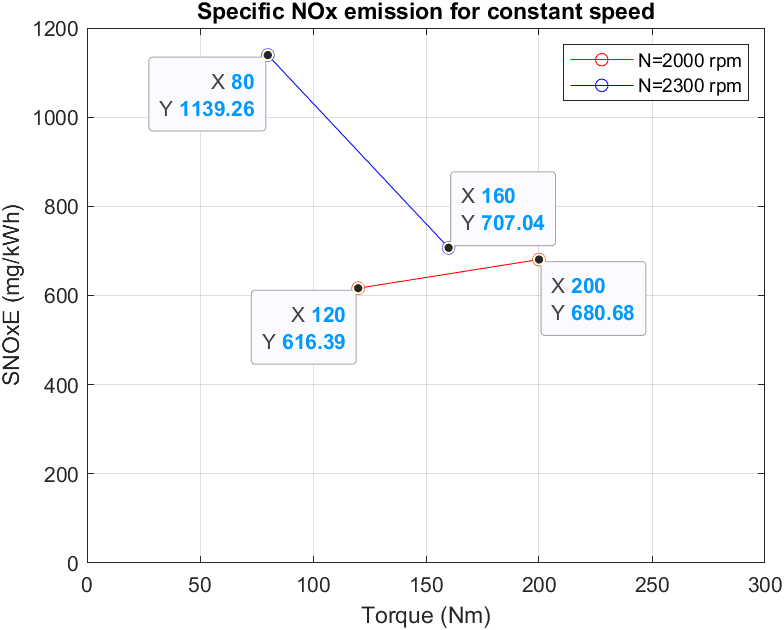
\includegraphics[width=.6\textwidth]{erwthma5a(diorthwsh).png} \caption{Ειδική εκπομπή $NO_x$ για σταθερό αριθμό στροφών} \label{fig:snoxe}\end{figure}\begin{figure}[!h]  \centering 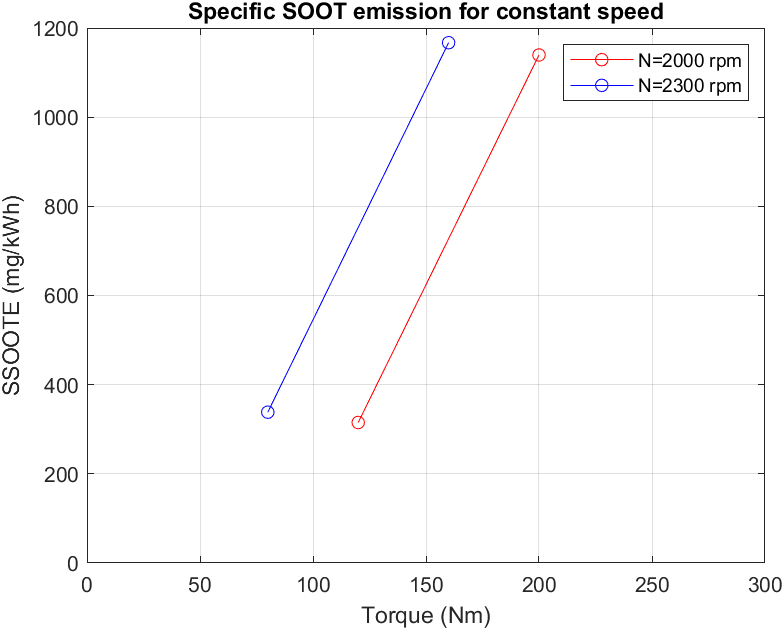
\includegraphics[width=.6\textwidth]{erwthma5b.png}  \caption{Ειδική εκπομπή $SOOT$ για σταθερό αριθμό στροφών}  \label{fig:ssoote}\end{figure}


\section{Question 5}

In the fifth and final question, the specific emissions of $NO_x$ and $SOOT$ are requested. Similar to the specific fuel consumption (Equation \ref{eq:SFC}), specific emissions can be defined as follows:

\begin{equation}
    \label{eq:SNOxE}
    SNO_xE=\frac{\dot{m}_{NO_x}}{P_e}\quad (mg/kWh)
\end{equation}

\begin{equation}
    \label{eq:SSOOTE}
    SSOOTE=\frac{\dot{m}_{SOOT}}{P_e}\quad (mg/kWh)
\end{equation}

To calculate these specific emissions, we need to first calculate the mass flows of pollutants. Based on the data in Table \ref{tab:metrhseis}, we have the concentration of $NO_x$ in parts per million (ppm). To convert this to $mg/h$, the following process is applied:

$$NOx\:(ppm)=\frac{n_{solute}\: (mol)}{n_{solution}\: (mol)}\times 10^6<=>$$

$$NOx\:(ppm)=\frac{\dot{n}_{solute}\: (mol/s)}{\dot{n}_{solution}\: (mol/s)}\times 10^6<=>$$

$$NOx\:(ppm)=\frac{\dot{n}_{NO_x}\: (mol/s)}{\dot{n}_{exhaust}\: (mol/s)}\times 10^6<=>$$

$$NOx\:(ppm)=\frac{\frac{\dot{m}_{NO_x}\: (kg/s)}{MB_{NO_x}\: (kg/mol)}}{\frac{\dot{m}_{exhaust}\: (kg/s)}{MB_{exhaust}\: (kg/mol)}}\times 10^6<=>$$

\begin{equation}
    \label{eq:m.NOx}
   \dot{m}_{NO_x}\: (kg/s)=\frac{\dot{m}_{exhaust}\: (kg/s)\cdot NO_x\:(ppm)\cdot MB_{NO_x}\: (kg/mol)}{MB_{exhaust}\: (kg/mol)}\times 10^{-6} 
\end{equation}

\begin{equation}
    \label{eq:m.NOx2}
   \dot{m}_{NO_x}\: (mg/h)= \dot{m}_{NO_x}\: (kg/s) \cdot 36\times 10^8
\end{equation}

Given the values of molecular weights, $MB_{NO_x}=0.0460055 \: kg/mol$ and $MB_{exhaust}=0.02898 \: kg/mol$, the values of the mass flow rate of $NO_x$ can be calculated as shown in Table \ref{tab:m.NO_x}.

\begin{table}[h]
    \centering
    \renewcommand{\arraystretch}{1.2} 
    \begin{tabular}{|c|c|c|c|}
    \hline
    \rowcolor{blue}
    $\#$ & $NO_x$ & $\dot{m}_{NO_x}$ & $\dot{m}_{NO_x}$\\
    \hline
    \rowcolor{gray}
    - & $ppm$ & $\times 10^{-6}\: kg/s$ & $mg/h$\\
    \hline
    1 & 70 & 4.303 & 15491.63\\
    \hline
    2 & 92 & 7.920 & 28512.31\\
    \hline
    3 & 94 & 6.098 & 21951.77\\
    \hline
    4 & 86 & 7.569 & 27247.13\\
    \hline 
    \end{tabular}
    \caption{Mass flow rate of $NO_x$ values for each operating point}
    \label{tab:m.NO_x}
\end{table}

Therefore, using Equation \ref{eq:SNOxE}, the specific emissions can be calculated from the mass flow rate of $NO_x$ ($mg/h$) and the power values from Table \ref{tab:finaltable3o}. The calculated specific emissions are shown in Table \ref{tab:finaltable5oa}.

\begin{table}[!h]
    \centering
    \renewcommand{\arraystretch}{1.2} 
    \begin{tabular}{|c|c|}
    \hline
    \rowcolor{blue}
    $\#$ & $SNO_xE$\\
    \hline
    \rowcolor{gray}
    - & $mg/kWh$\\
    \hline
    1 & 616.39\\
    \hline
    2 & 680.68\\
    \hline
    3 & 1139.26\\
    \hline
    4 & 707.04\\
    \hline 
    \end{tabular}
    \caption{Specific emissions of $NO_x$ for the operating points}
    \label{tab:finaltable5oa}
\end{table}

To calculate the specific emissions of $SOOT$, we need to determine the mass flow rate again. It is known from Thermodynamics that a gas mixture can be considered as a new ideal gas. Thus, the exhaust gas mixture can be considered an ideal gas for which the Ideal Gas Equation is written as:

$$P\cdot V=n\cdot R\cdot T<=>$$

$$P=\frac{\rho_{exhaust}}{MB_{exhaust}}\cdot R\cdot T_{exhaust}<=>$$
 
$$\rho_{exhaust}=\frac{P\cdot MB_{exhaust} }{R\cdot T_{exhaust}}$$

where:
\begin{itemize}
 \item $\boldsymbol{P}$ is the pressure at which the exhaust gas is located, and it is equal to atmospheric pressure, $10^5\: Pa$
\item $\boldsymbol{R}$ is the universal gas constant for gases, and it is equal to $8.3145\: J/mol\cdot K$
\item $\boldsymbol{MB_{exhaust}}$ is the molecular weight of the exhaust gas, given as $28.98\: kg/kmol$
\item $\boldsymbol{T_{exhaust}}$ is the temperature at which the exhaust gas is located for each operating point and is given by measurements
\end{itemize}
Summarizing, we have:

$$\rho_{exhaust}=\frac{10^5\: (Pa)\cdot 28.98\: (kg/kmol)}{8.3145\times 10^{-3}\: (J/kmol\cdot K)\cdot T_{exh}}$$

or finally:

\begin{equation}
    \label{eq:rhoexh}
    \rho_{exhaust}=\frac{348.548}{T_{exh}}\: (kg/m^3)
\end{equation}

So, from Table \ref{tab:metrhseis} and Equation \ref{eq:rhoexh}, the density of the exhaust gas is calculated at each operating point. Then, by dividing these values by the mass flow rates of the exhaust gas from Table \ref{tab:m.exh}, the volumetric flow rates of the exhaust gas are obtained according to the equation:
$$\dot{V}_{exhaust}\: (m^3/s)=\frac{\dot{m}_{exhaust}\: (kg/s)}{\rho_{exhaust}\: (kg/m^3)}$$

These values are shown in Table \ref{tab:V.exh}.

\begin{table}[h]
\centering
\renewcommand{\arraystretch}{1.2}
\begin{tabular}{|c|c|c|c|}
\hline
\rowcolor{blue}
$\#$ & $\rho_{exhaust}$ & $\dot{m}_{exhaust}$ & $\dot{V}_{exhaust}$\\
\hline
\rowcolor{gray}
- & $kg/m^3$ & $kg/s$ & $m^3/s$\\
\hline
1 & 0.52810 & 0.03872 & 0.073328\\
\hline
2 & 0.47037 & 0.05423 & 0.115289\\
\hline
3 & 0.58678 & 0.04086 & 0.069639\\
\hline
4 & 0.48816 & 0.05544 & 0.113565\\
\hline
\end{tabular}
\caption{Values of density, mass flow rate, and volume flow rate of the exhaust gas for each operating point}
\label{tab:V.exh}
\end{table}

Since the pollutant is contained in the exhaust gas flow rate $\dot{V}_{exhaust}$, we have:
$$\dot{m}_{SOOT}\: (mg/s)=SOOT\: (mg/m^3)\cdot \dot{V}_{exhaust}\: (m^3/s)<=>$$

\begin{equation}
\label{eq:m.soot}
\dot{m}_{SOOT}\: (mg/h)=3600\cdot SOOT\: (mg/m^3)\cdot \dot{V}_{exhaust}\: (m^3/s)
\end{equation}

With the given density of $SOOT$ in $mg/m^3$ (from the measurements in Table \ref{tab:metrhseis}), from Table \ref{tab:V.exh} and Equation \ref{eq:m.soot}, the mass flow rate values of the pollutant are obtained.

Finally, using Equation \ref{eq:SSOOTE} and for the known power values, the requested specific emissions are obtained in Table \ref{tab:finaltable5ob}.

\begin{table}[h]
\centering
\renewcommand{\arraystretch}{1.2}
\begin{tabular}{|c|c|c|}
\hline
\rowcolor{blue}
$#$ & $\dot{m}_{SOOT}$ & $SSOOTE$\\
\hline
\rowcolor{gray}
- & $mg/h$ & $mg/kWh$\\
\hline
1 & 7919.37 & 315.10\\
\hline
2 & 47729.51 & 1139.46\\
\hline
3 & 6518.20 & 338.28\\
\hline
4 & 44971.73 & 1166.98\\
\hline
\end{tabular}
\caption{Values of mass flow rate and specific emission $SOOT$ for each operating point}
\label{tab:finaltable5ob}
\end{table}
\newpage

Finally, in Figures \ref{fig:snoxe} and \ref{fig:ssoote}, the specific emissions of pollutants $NO_x$ and $SOOT$ are shown as functions of torque for a constant number of revolutions. It can be observed that for a \textbf{constant} number of revolutions $N$ and as torque $M$ \textbf{increases}, the specific emission $SOOT$, $SSOOTE$, \textbf{increases}. Also, for a \textbf{constant} number of revolutions $N=2000\: rpm$ and as torque $M$ \textbf{increases}, the specific emission $NO_x$, $SNO_xE$, \textbf{increases}, while for a \textbf{constant} number of revolutions $N=2300\: rpm$, it decreases.

\begin{figure}[!h]
\centering
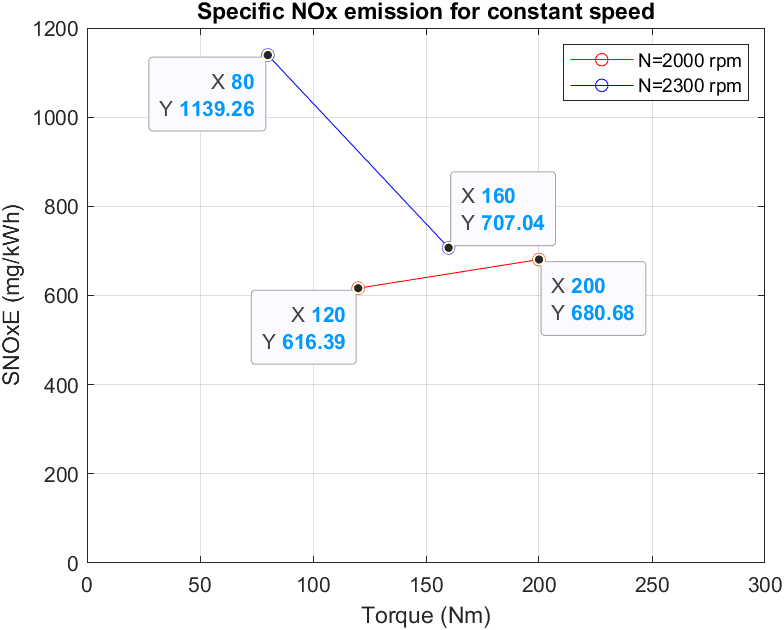
\includegraphics[width=.6\textwidth]{erwthma5a(diorthwsh).png}
\caption{Specific emission $NO_x$ for a constant number of revolutions}
\label{fig:snoxe}
\end{figure}

\begin{figure}[!h]
\centering
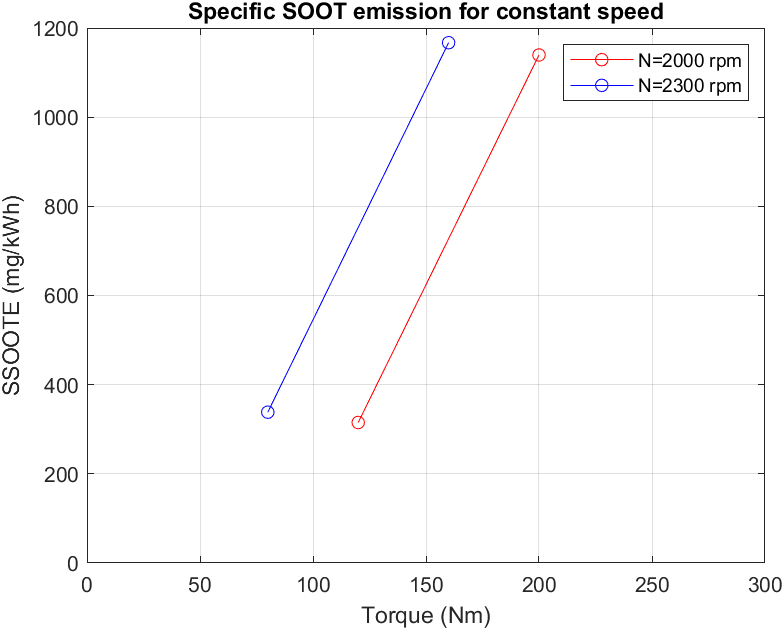
\includegraphics[width=.6\textwidth]{erwthma5b.png}
\caption{Specific emission $SOOT$ for a constant number of revolutions}
\label{fig:ssoote}
\end{figure}










%\chapter{Συμπεράσματα}Με το πέρας της μελέτης αυτής τα συμπεράσματα που προκύπτουν είναι τα εξής\begin{enumerate} \item Παρατηρώντας το Σχήμα \ref{fig:m./Torque} φαίνεται ότι κρατώντας το $Ν$ σταθερό, για μεγαλύτερες ροπές εμφανίζεται μικρότερη παροχή ψυκτικού. Επομένως σε πιο υψηλές ροπές του κινητήρα δεν υπάρχει τόσο μεγάλη ανάγκη για ψύξη και κατ' επέκταση ο κινητήρας ζορίζει το σύστημα ψύξης περισσότερο για χαμηλές τιμές της ροπής $M$. Τέλος παρατηρείται επίσης ότι αυξάνοντας τον αριθμό στροφών $N$ μειώνεται ο η παροχή του ψυκτικού και έτσι, αντίστοιχα στους χαμηλότερους αριθμούς στροφών υπάρχει μικρότερη ανάγκη για ψύξη. \item Παρατηρώντας το Σχήμα \ref{fig:isolfig} φαίνεται ότι κρατώντας το $N$ σταθερό, για μεγαλύτερες ροπές εμφανίζονται μεγαλύτερα μεγέθη ισχύος. Επόμενως σε πιο υψηλές ροπές του κινητήρα προσδίδεται μεγαλύτερη τιμή ενέργειας στο καύσιμο ($\dot{Q}_{fuel}$ αυξάνεται). Επίσης, μπορεί κανείς να δει ότι για ότι για μικρότερο αριθμό στροφών τα μεγέθη της ισχύος μειώνονται. Τέλος φαίνεται ότι το μεγαλύτερο μέρος της προσδιδόμενης ενέργειας στο καύσιμο την προσφέρει η πραγματική ισχύς του κινητήρα $P_e$, έπειτα η ισχύς του ψυκτικού $\dot{Q}_{coolant}$, η ισχύς του καυσαερίου $\dot{Q}_{exhaust}$ και τέλος οι άδηλες απώλειες $\dot{Q}_A$. Φαίνεται δηλαδή πως γενικά ισχύει: $$\dot{Q}_{fuel}>P_e>\dot{Q}_{coolant}>\dot{Q}_{exhaust}>\dot{Q}_A$$\item Από το Σχήμα \ref{fig:SFC/eta} παρατηρείται ότι κρατώντας το $N$ σταθερό, για μεγαλύτερες ροπές εμφανίζονται μικρότερα μεγέθη ειδικής κατανάλωσης καυσίμου $SFC$ και μεγαλύτερα βαθμού απόδοσης $\eta$. Επομένως για μεγαλύτερες ροπές του κινητήρα φαίνεται πως καταναλώνεται λιγότερο καύσιμο. Δηλαδή ο κινητήρας ζορίζεται περισσότερο σε χαμηλές ροπές. Αντίθετα για τον βαθμό απόδοσης. Έτσι λοιπόν, ο κινητήρας αποδίδει καλύτερα σε μεγάλες ροπές αλλά καταναλώνει περισσότερο καύσιμο. Τέλος, από την σχέση \ref{eq:sfc/eta} αντιλαμβάνεται κανείς ότι τα μεγέθη του βαθμού απόδοσης $\eta$ και της ειδικής κατανάλωσης καυσίμου $SFC$ είναι αντιστρόφως ανάλογα: $$\eta\propto\frac{1}{SFC}$$ \item Παρατηρείται από το Σχήμα \ref{fig:AFR} πως κρατώντας το $N$ σταθερό, για μεγαλύτερες ροπές εμφανίζεται μικρότερος λόγος ισοδυναμίας αέρα-καυσίμου $AFR$. Αυτό συνεπάγεται ότι αυξανόμενης της ροπής, η παροχή μάζας του αέρα μειώνεται σε σχέση με την παροχή μάζας καυσίμου. Επομένως καίγεται λιγότερος αέρας σε χαμηλές ροπές του κινητήρα. Τέλος, φαίνεται ότι για μικρότερο αριθμό στροφών ο λόγος αυτός μειώνεται εν γένει.\item Στο Σχήμα \ref{fig:ssoote} φαίνεται ότι κρατώντας το $N$ σταθερό, για μεγαλύτερες ροπές εμφανίζεται μεγαλύτερη ειδική εκπομπή αιθάλης $SSOOTE$. Άρα, σε μεγαλύτερες ροπές του κινητήρα εκπέμπεται περισσότερο $SOOT$ στην ατμόσφαιρα. Επίσης παρατηρεί κανείς ότι για μικρότερο αριθμό στροφών γενικά αυξάνεται η εκπομπή της αιθάλης.\newline Από το Σχήμα \ref{fig:snoxe} δεν μπορούν να προκύψουν συμπεράσματα για την μεταβολή της ειδικής εκπομπής $NO_x$ για σταθερό αριθμό στροφών. Ωστόσο θα μπορούσε ίσως να γίνει η εικασία ότι από μια τιμή των στροφών και άνω, το $SNO_xE$ αυξάνεται, αυξανόμενης της ροπής του κινητήρα, ενώ από έναν αριθμό στροφών και κάτω αντίστροφα. Τέλος παρατηρείται ότι για μεγαλύτερους αριθμούς στροφών η ειδική εκπομπή $NO_x$ αυξάνεται εν γένει.\end{enumerate}\newpage



\chapter{Conclusions}

Upon completing this study, the following conclusions can be drawn:
\begin{enumerate}
    \item Observing Figure \ref{fig:m./Torque}, it appears that keeping $N$ constant, higher torques result in lower coolant flow rates. Therefore, for higher engine torques, there is less need for cooling, and consequently, the engine strains the cooling system more for lower torque values $M$. Additionally, it is also observed that increasing the number of revolutions $N$ decreases the coolant flow rate, indicating less need for cooling at lower RPMs.
    \item Observing Figure \ref{fig:isolfig}, it is evident that keeping $N$ constant, higher torques correspond to higher power values. Thus, for higher engine torques, more energy is added to the fuel ($\dot{Q}_{fuel}$ increases). Furthermore, one can see that power values decrease for lower RPMs. Finally, it is noted that most of the energy is contributed to the fuel by the actual engine power $P_e$, followed by coolant power $\dot{Q}_{coolant}$, exhaust gas power $\dot{Q}_{exhaust}$, and lastly, the losses $\dot{Q}_A$. It generally holds that: $$\dot{Q}_{fuel}>P_e>\dot{Q}_{coolant}>\dot{Q}_{exhaust}>\dot{Q}_A$$
    \item From Figure \ref{fig:SFC/eta}, it is observed that keeping $N$ constant, higher torques result in lower specific fuel consumption values $SFC$ and higher efficiency values $\eta$. Therefore, for higher engine torques, less fuel is consumed. The engine works harder at lower torques. Conversely, for efficiency, the engine performs better at higher torques but consumes more fuel. Finally, from equation \ref{eq:sfc/eta}, it is understood that the efficiency $\eta$ and specific fuel consumption $SFC$ are inversely proportional:
    $$\eta\propto\frac{1}{SFC}$$
    \item In Figure \ref{fig:AFR}, it is noticed that keeping $N$ constant, higher torques correspond to lower air-fuel ratio values $AFR$. This implies that with increasing torque, the air mass flow decreases compared to the fuel mass flow. Therefore, less air is burned at low engine torques. Finally, it is observed that this ratio generally decreases for lower RPMs.
    \item In Figure \ref{fig:ssoote}, it is evident that keeping $N$ constant, higher torques result in higher specific SOOT emission values $SSOOTE$. Thus, at higher engine torques, more SOOT is emitted into the atmosphere. Also, it can be seen that, in general, emissions of soot increase for lower RPMs. From Figure \ref{fig:snoxe}, no conclusions can be drawn about the variation of specific nitrogen oxide emissions $NO_x$ for a constant number of revolutions. However, it could be speculated that beyond a certain RPM value, $SNO_xE$ increases with increasing engine torque, while below a certain RPM, it decreases. Finally, it is observed that, in general, specific $NO_x$ emissions increase for higher RPMs.
\end{enumerate}
\newpage








\listoffigures
\begingroup
\let\clearpage\relax
\listoftables
\endgroup










 \newpage


\printbibliography[title=References]

\nocite{cengel2011thermodynamics}
\nocite{wiki:Gas_constant}
\nocite{wiki:Brake-specific_fuel_consumption}
\nocite{libretexts1503Solution}








\end{document}